%% Example file for a masterthesis
% Copyright 2010 by Dirk Willrodt <dwillrodt@zbh.uni-hamburg.de>
% --------------------------------------------------------------
%
% This file may be distributed and/or modified under the
% conditions of the LaTeX Project Public License, either version 1.2
% of this license or (at your option) any later version.
% The latest version of this license is in:
%
%    http://www.latex-project.org/lppl.txt
%
% and version 1.2 or later is part of all distributions of LaTeX
% version 1999/12/01 or later.
%
% Usage: just compile it with pdflatex, and see how it looks, and what caused
% this. You can also take it and change blocks marked like this:
%%%%>
% ...
%%%%<
% to produce Your own thesis.
%
% check chapters in sub folders for examples of usage of different mark-ups


% use the option ger for thesis in german.
% use the option bsc for a bachelor thesis.
% you can pass options to scrreprt, for example numbers=noenddot for if you have
% an appendix and you don't want '.' at the end of chapter numbers
%\documentclass[twoside,a4paper,ger,bsc]{master}
\documentclass[twoside,a4paper,bsc]{master}
%%%%>
% the following package is only needed to produce dummy text.
% You do not need it for your thesis.
%\usepackage{lipsum}
% This package is not included in the class, because it is not needed, but we
% recommend to use it. It only works with pdfLaTeX.
\usepackage[kerning,spacing]{microtype}

% add other packages, as needed.
\usepackage{amsmath}
\usepackage{amsfonts}
\usepackage{mathtools}
\usepackage{graphicx}
\usepackage{pdfpages}
\usepackage{algpseudocode}
\usepackage{algorithm}
\usepackage{palatino}
\usepackage{numprint}
\usepackage{svg}
\usepackage{comment}
\usepackage{float}
\usepackage{times}
\usepackage{theorem}
\usepackage{tikz}
\usepackage{amssymb}
\usepackage{dcolumn}

\usetikzlibrary{chains}
\usetikzlibrary{decorations.pathmorphing}
\usepgflibrary{decorations.pathreplacing}
\usetikzlibrary{decorations.text}

%%%Comment macro
\newcounter{mycommentcounter}
\newcommand{\Genericcomment}[2]{%
\par%
\noindent%
\fbox{%
\begin{minipage}{0.95\textwidth}
\textsl{#1: \#\refstepcounter{mycommentcounter}%
\arabic{mycommentcounter}: #2}%
\end{minipage}%
}%
\par%
}


\newcommand{\AVTcomment}[1]{
\Genericcomment{AVT}{#1}
}

\newcommand{\SKcomment}[1]{
\Genericcomment{SK}{#1}
}

%%% Other macros
\newcommand{\Qgram}[1]{\(#1\)-gram}
\newcommand{\Seed}[0]{\mathsf{seed}}
\newcommand{\Span}[0]{\mathsf{span}}
\newcommand{\InBlock}[0]{\mathsf{inBlock}}
\newcommand{\True}[0]{\mathsf{true}}
\newcommand{\False}[0]{\mathsf{false}}
\newcommand{\Rank}[0]{\mathsf{rank}}
\newcommand{\Blocks}[0]{\mathsf{blocks}}
\newcommand{\Block}[0]{\mathsf{block}}
\newcommand{\CharToAdd}[0]{\mathsf{CharToAdd}}
\newcommand{\PosToAdd}[0]{\mathsf{PosToAdd}}
\newcommand{\CharToRmv}[0]{\mathsf{CharToRmv}}
\newcommand{\PosToRmv}[0]{\mathsf{PosToRmv}}
\newcommand{\RankToAdd}[0]{\mathsf{RankToAdd}}
\newcommand{\RankToRmv}[0]{\mathsf{RankToRmv}}
\newcommand{\Query}[0]{\mathsf{Query}}
\newcommand{\Target}[0]{\mathsf{Target}}
\newcommand{\Append}[0]{\mathsf{append}}
\newcommand{\QueryIdx}[0]{\mathsf{QueryIdx}}
\newcommand{\TargetIdx}[0]{\mathsf{TargetIdx}}
\newcommand{\Start}[0]{\mathsf{start}}
\newcommand{\End}[0]{\mathsf{end}}
\newcommand{\TBlockEnd}[0]{\mathsf{TargetBlockEnd}}
\newcommand{\QBlockEnd}[0]{\mathsf{QueryBlockEnd}}
\newcommand{\HashValue}[0]{\mathsf{HashValue}}
\newcommand{\HashValVec}[0]{\mathsf{HashValVec}}
\newcommand{\CurrentWeight}[0]{\mathsf{CurrentWeight}}
\newcommand{\SuffixCode}[0]{\mathsf{SuffixCode}}
\newcommand{\Code}[0]{\mathsf{code}}
\newcommand{\Score}[0]{\mathsf{score}}
\newcommand{\Loopid}[0]{\mathsf{loopid}}
\newcommand{\Wheel}[0]{\mathsf{wheel}}
\newcommand{\IT}[2]{\mathsf{IndexTable}_{#1,#2}}
\newcommand{\LE}[2]{\mathsf{LinearEnc}_{#1,#2}}
\newcommand{\Small}[0]{\mathsf{small}}
\newcommand{\Biggg}[0]{\mathsf{big}}
\newcommand{\DivFactors}[0]{\mathsf{divFactors}}
\newcommand{\DivFactor}[0]{\mathsf{divFactor}}
\newcommand{\ModFactors}[0]{\mathsf{modFactors}}
\newcommand{\PossibleValuesSingle}[0]{\mathsf{possibleValuesSingle}}
\newcommand{\PossibleValuesTotal}[0]{\mathsf{possibleValuesTotal}}
\newcommand{\Psum}[0]{\mathsf{psum}}
\newcommand{\Cutoff}[0]{\mathsf{cutoff}}
\newcommand{\Substring}[3]{#1\lbrack #2\ldots#3\rbrack}
\newcommand{\Subchar}[2]{#1\lbrack #2\rbrack}
\newcommand{\Scoretablename}[0]{\mathsf{ST}}
\newcommand{\Scoretable}[2]{\Scoretablename_{#1}[#2]}
\newcommand{\Reals}{\mathbb{R}}
\newcommand{\Permname}[1]{\varphi_{#1}}
\newcommand{\Perm}[2]{\Permname{#1}(#2)}
\newcommand{\Permnameinverse}[1]{\varphi_{#1}^{-1}}
\newcommand{\Perminverse}[2]{\Permnameinverse{#1}(#2)}
\newcommand{\Alpha}[0]{\mathcal{A}}
\newcommand{\Nats}{\mathbb{N}}
\newcommand{\Qsplit}{\mathsf{QS}}

\theorembodyfont{\rmfamily}
\theoremheaderfont{\rmfamily\bfseries}
\newcounter{Lemmacounter}
\newtheorem{myLemma}[Lemmacounter]{Lemma}
\newcommand{\AfterNumber}{}
\newcommand{\Skiptheorem}{\smallskipamount}
\newcommand{\StartFormal}[1]{\par\addvspace{\Skiptheorem}\noindent\textbf{#1}}
\newcommand{\EndFormal}{\par\addvspace{\Skiptheorem}}
%\newenvironment{Lemma}{\begin{myLemma}\AfterNumber}{\end{myLemma}}
\newenvironment{Proof}{\StartFormal{Proof:}}{\EndFormal}
\def\FirstMultisetSymbol{\(a_0\)}
\def\SecondMultisetSymbol{\(a_1\)}
\def\ThirdMultisetSymbol{\(a_2\)}

%%%%<

% Helpfull command to put reminders in your work
\newcommand{\Todo}[1]%
{\colorbox{orange}{\mbox{}\\\fbox{\parbox{\textwidth}{\textbf{Todo: #1}}}}\\}
% it uses one argument which is referred to by #1

\begin{document}

% use roman page numbers before the real document starts.
\pagenumbering{roman}

%Change the values here to get your title page and assertion page right
\AdvisorA{Stefan Kurtz}
\AdvisorB{Andrew Torda}
\author{Anh Viet Ta}
\MatrikelNo{\numprint{6747004}}
%\AuthorAdress{Musterstrasse 1}{07770 M\"unchhausen}
\title{
       \begin{tabular}{c}
       \textbf{Efficient Preprocessing of Short Sequence Segments}\\[3mm]
       \textbf{for Efficient Filtering in Comparing Protein Sequences}
       \end{tabular}}
% add data line or leave it to use current date.
%\date{1.4.2016}
\Maketitle

\SKcomment{Please provide a longer abstract}

% if you write in German, maybe change this to "Zusammenfassung".
\addchap*{Abstract}
\small
%%%%>
In analysis of protein and DNA sequences, the concept of homology is
central. It
may suggest that organisms share a common evolutionary ancestor when two
sequences or structures share more similarity than expected by chance. But
in
reality, homologous sequences do not always share significant sequence
similarity but instead their resemblances are based on statistically
significant
structure likeness or a connection to a intermediate sequence. There rises
a
need for algorithms not only to find exact matches in sequences, but also
to
find local similarities (sensitive searching) and cluster them into groups
(sequence clustering).
The software suite MMseqs2 and its predecessor MMseqs are the new standard
of both sensitive biological sequence searching and sequence clustering.
The prefiltering module in MMseqs2 is of particular importance, since it
serves to rapidly reduce possibility space. This thesis focusses on the
first phase of the filtering approach, i.e.\ the construction of the
\(k\)-environment and shows how to systematically improve its runtime and
space requirement.
%%%%<
\normalsize
% The first sets the depth of the TOC, the second produces it. Change the
% number if you need a ``deeper'' TOC.
\setcounter{tocdepth}{1}
\tableofcontents
%%%%>
% include chapters from subfolders
% change if you need more chapters or if you want to call them different,
this
% is just an example
\Chapter{Introduction}
\section{Recent developments of bioinformatic sequence searching and
clustering}
% reset to arabic page numbers will start with 1
\pagenumbering{arabic}
With the advent of high-throughput sequencing technologies, the cost of
sequencing DNA has dramatically be reduced. Sequence databases, such as
UniProt have been growing by a factor of two every two
years~\cite{apweiler2004uniprot}, which leads to a significant focus on
developing searching and clustering methods that can handle large-scale
datasets
efficiently.
On sequence searching, new algorithms and heuristics have been developed to
improve sensitivity without sacrificing speed. Tools like
DIAMOND~\cite{buchfink2015fast,BUC:REU:DRO:2021} and
MMseqs2~\cite{steinegger2017mmseqs2} provide fast and sensitive sequence
searching capabilities,
especially in metagenomics and large-scale sequencing projects.
Hidden
Markov Model based
methods, such as the HMMER~\cite{finn2011hmmer} software, have been
enhanced to improve their
sensitivity and accuracy, making them invaluable for protein domain and
family searching. The existing algorithms like BLAST have also seen massive
improvement by using GPU parallelization~\cite{vouzis2011gpu} and specific
hardwares, namely
FPGAs (Field-Programmable Gate Arrays)~\cite{guo2012systolic} have been
customized for
accelerating sequence searching algorithms.
Recent developments on metagenomics have also given ways to specialized
databases and algorithms. These databases contain sequences from
environmental samples and enable the identification of novel organisms and
genes within complex microbial communities.
On sequence clustering, myriads of methods have been developed. Graph-based
clustering methods, such as Markov Clustering
(MCL)~\cite{shih2012identifying} and the
Louvain~\cite{rahiminejad2019topological} algorithm,
have gained popularity. These methods model sequences as nodes in a graph
and use edge weights to represent similarities, allowing for the detection
of densely connected clusters within the graph. Density-based methods like
DBSCAN~\cite{ester1996density} (Density-Based Spatial Clustering of
Applications with Noise) have
seen applications in bioinformatics~\cite{karim2021deep}. These algorithms
group sequences based on
the density of data points, enabling the discovery of clusters with varying
shapes and sizes. Traditional distance-based clustering algorithms, such as
hierarchical clustering~\cite{lafond2017new} and
k-means~\cite{hussain2011fpga}, have been adapted and optimized for
large biological datasets.
\section{MMseqs2}
MMseqs~\cite{hauser2014mmseqs} (Many-against-Many sequence searching) is a
software suite for fast
and deep clustering and searching of large datasets.
It consists of three core modules:
\begin{itemize}
\item a fast and sensitive prefiltering module
that eliminates most non-homologous sequences,
\item a local alignment module based on the Smith-Waterman algorithm
using the ideas and implementation techniques described
in~\cite{Farrar:2007hs,ZHA:LEE:GAR:MAR:2013},
\item and a clustering module based on a
similary graph.
\end{itemize}
Due to the modularity of the structure, it allows users to
create workflows tailored to specific clustering and searching needs. The
default workflow utilizes the UniProt databases to create predefined
parameters and resembles the average use case. The second, cascaded
clustering, clusters the input database in multiple steps, increasing the
sensitivity between each steps and therefore enables finding
best-hit-searches 4-10 times faster compared to default workflow.
The third workflow simply compares
databases using only prefiltering and aligning modules. The last workflow
updates clustering between new and old clustered database by deleting
deprecated sequences and appending new sequences to each cluster.
In benchmarks, MMseqs showed to be 4-30 times faster than
UBLAST~\cite{edgar2010search} and RAPsearch2~\cite{zhao2012rapsearch2}.
MMseqs could cluster large databases down to 30\% sequence
identity \numprint{2000} times faster than BLASTclust.
An improved, updated version MMseqs2~\cite{steinegger2017mmseqs2} was
published in 2017.
It provides dramatic improvements in both efficiency and sensitivity by
introducing several novel ideas:
\begin{itemize}
\item The prefiltering stage was revamped by
introducing an algorithm to find two consecutive, spaced-seed \Qgram{q}
matches
and optimizing memory access.
\item Extension to allow the usage of \Qgram{7} due to
the speedup of the algorithm.
\item Integration of MPI (Message-Passing-Interface) allows the
distribution of jobs on computer clusters.
\item Iterative profile search increases sensitivity far greater
than sensitivity of BLAST.
\end{itemize}
An in-depth look into the three core modules is presented below.
\SKcomment{I will skip reading the next section.}
\subsection{Fast \Qgram{q} prefiltering stage}
In MMseqs, the prefiltering stage is the first step to process all
sequences and serves to reduce the search space significantly, therefore
it's imperative for the algorithm to be as efficient as possible. The
process consists of 4 loops as outlined in
Figure~\ref{fig:prefilterMMseqs}. In the first loop, query sequences are
searched one by one against the target set. For each spaced seed window in
the query sequence (loop 2), a \Qgram{q} is extracted and a list of all
similar \Qgram{q}s with a Blosum62 similarity above a threshold score is
created using a linear-time branch-and-bound algorithm. Lower threshold
scores result in higher average numbers of similar k-mers and thereby
higher sensitivity and lower speed. Each generated \Qgram{q} (loop 3) then
gets queried against a precomputed database of \Qgram{q}s in target
sequences. The sum of scores of the corresponding target sequences then
gets collected in a vector based on the prefiltering score. In the last
step the target score vector is sorted and the best matches get processed
further.
\begin{figure}[t]
\begin{center}
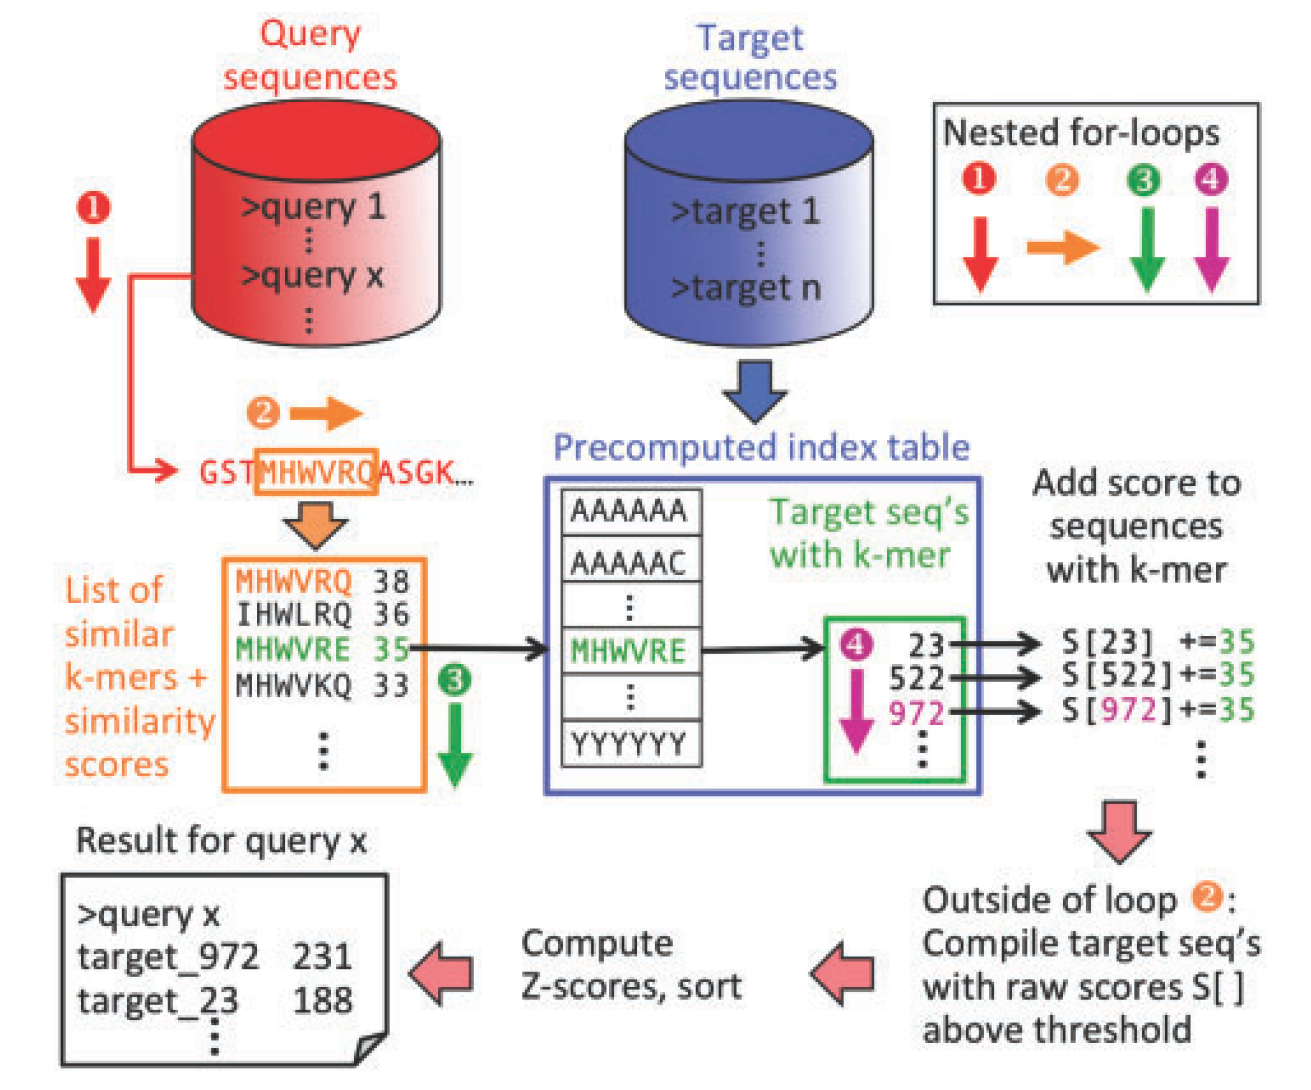
\includegraphics[scale=0.3]{graphics/MMseqs_prefilter.png}
\end{center}
\caption{Prefiltering stage in MMseqs~\cite{hauser2014mmseqs}}
\label{fig:prefilterMMseqs}
\end{figure}
In MMseqs2, the prefiltering stage was reengineered (See
Figure~\ref{fig:prefilterMMseqs2}). After the query-target matches are
collected, they get sorted and iterated over to detect double k-mer matches
by comparing the current diagonal with the previously matched diagonal. If
the previous and current diagonals agree, they both get stored as a double
match for the ungapped alignment stage.
\begin{figure}[t]
\begin{center}
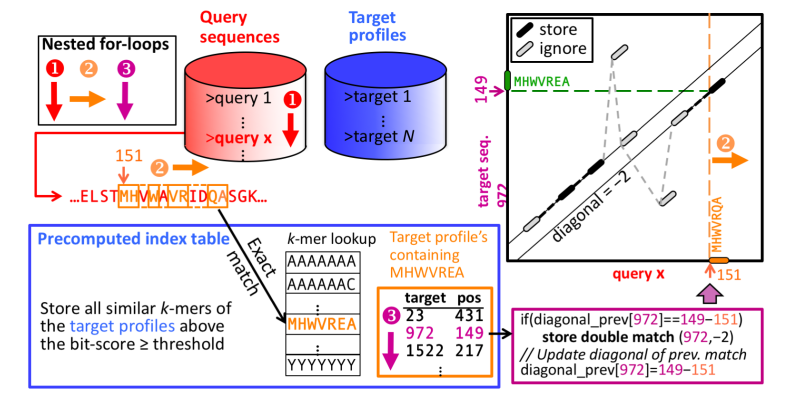
\includegraphics[scale=0.7]{graphics/MMseqs2_prefilter.png}
\end{center}
\caption{Prefiltering stage in MMseqs2~\cite{steinegger2017mmseqs2}}
\label{fig:prefilterMMseqs2}
\end{figure}
\subsection{Ungapped alignment and Smith-Waterman alignment stage}
In MMseqs2, an additional ungapped alignment stage was introduced, where
many target sequences are aligned at once using a vectorized approach. It
also utilizes a linear memory access using a score matrix containing the p.
Due to the extensive use of SIMD instructions, this stage achieves a linear
time complexity, much more efficient compared to the Smith-Waterman
alignment stage.
After the ungapped alignment is completed, MMseqs2 computes for all
filtered
query-target sequence pairs an exact, unbounded Smith-Waterman alignments
with affine gap penalties. This module utilizes a highly vectorized
algorithm
equipped with new SIMD instructions and adapted for sequence profiles.
\Chapter{Methods}
For every alphabet \(\Alpha\), we can define a bijective mapping to a
subset
of \(\Nats\) of size \(|\Alpha|\). Therefore, in the
following sections we consider sequences over \(\Alpha\) as sequences of
integers, where each integer encodes a different character of \(\Alpha\).
That is, the alphabet will be interpreted mostly as an integer
subset \([0,|\mathcal{A}|)\cap \Nats\).
\section{Efficient enumeration of hash values}
Since the database can be very large, a precise and efficient enumeration
of
hash values in every sequence position must be prioritized. In MMseqs2, at
every residue,
relevant characters based on the user-chosen spaced seed, which weight is
denoted by \(q\), are individually
extracted from the target sequence to create \Qgram{q}s and then process
these \Qgram{q}s as independent strings. This approach requires to compute
a hash value for each \Qgram{q} using \(O(q)\) time.For a sequence of
length
\(n\), this would sum up to \(O((n-q+1)q)=O(nq)\). This process is detailed
in
Algorithm~\ref{code:mmseqshash}.
\begin{algorithm}[t]
\caption{Hash enumeration in MMseqs2}
\label{code:mmseqshash}
\begin{tabular}{@{}l@{~}l}
\textbf{Input:}
&spaced seed \(\Seed\)\\
&Encoded sequence \(s\) of length \(n\)\\
&radix \(r = |\Alpha|\)
\end{tabular}
\begin{algorithmic}
\State \(\HashValVec\gets []\)
\For{\(j\) \textbf{from} 0 to $n-q$}\Comment{Iterate over sequence}
\State \(\HashValue \gets 0\)
\For{\(i \in [0,\Seed.\Span)\)}\Comment{Iterate over seed}
\If{\(\Seed[i]\)}
\State \(\HashValue\text{ = }\HashValue\cdot r\text{ + }s[j\text{ + }i]\)
\EndIf
\EndFor
\State \(\HashValVec .\Append(\HashValue)\)
\EndFor
\State return \(\HashValVec\)
\end{algorithmic}
\end{algorithm}
In order to optimize this process, a recursive hashing
algorithm~\cite{cohen1997recursive} could be implemented, where the spaced
seeds
are considered as a shifting hash window. To gather the next hash value,
the
window can be shifted by one, resulting in the removal and addition of old
and
new characters respectively, which are both determined by the spaced seed.
If
the spaced seed can be maximally divided into \(b\) blocks of consecutive
1s,
the \(b\) old characters can be characterized as the start of each block,
and
the new character respectively as the character directly after the end of
the
block. This schema is visualized in Figure~\ref{fig:recursive}.
\SKcomment{I assume that you have defined a block as a maximum sequence of
1-bits of a spaced seed. But then the new character directly after the end
of the block would correspond to a 0 bit in the spaced seed, i.e.\ it is
irrelevant
for the. Deducing this, This does not make sense.}
\AVTcomment{I'm accounting for the new character after shifting the window,
e.g
\(c\) in Figure~\ref{fig:recursive}.}
\begin{figure}[t]
\begin{center}
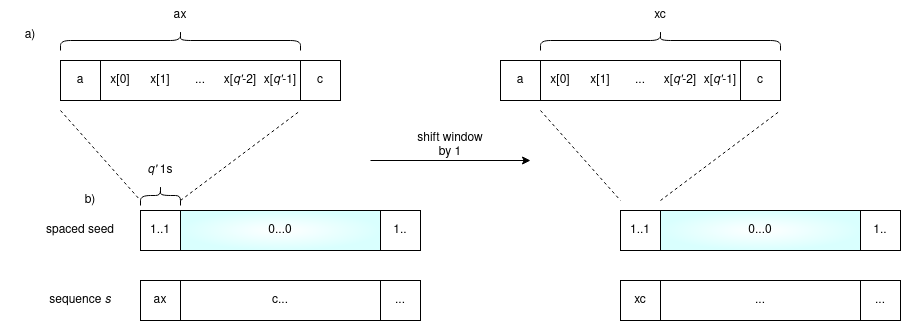
\includegraphics[scale=0.6]{graphics/recursive.png}
\end{center}
\caption{a) Schema of invertible integer hashing and b) decomposition of
spaced
seed into blocks of consecutive \Qgram{q}}
\label{fig:recursive}
\end{figure}
\SKcomment{You need to give more explanation for Figure 3.1. Also the
figure
suggests that the prefix of length \(q-1\) corresponds to the initial
block 1-bits. But \(q\) is the total number of 1-bits in the spaced seed.
As a consequence, the figure is misleading.}
\AVTcomment{To be fixed.}
\SKcomment{Unclear what you by this 'family of hash functions'? You likely
mean incremental/recursive hash functions?}
\AVTcomment{Fixed.}
\SKcomment{Please explain how you have fixed this.}
\AVTcomment{by this 'family of hash functions', I meant recursive hash
functions. I fixed it by rewording the section, naming recursive hash
function
at beginning of paragraph.}
Assuming the removal and addition operations on characters are of constant
time
complexity, the algorithm would run in \(O(nb)\) time, where \(b\) is the
number
of consecutive \Qgram{q} blocks. The simplest case of the algorithm, where
the
spaced seed itself is a consecutive \Qgram{q} (\(b=1\)), is called
invertible
integer hashing~\cite{gsa}, and it employs two fundamental equations.
In order to achieve independence between hash values, the characters are
usually
assigned a weight, which might be expressed as \(r^{q-1-i}\), where \(r\)
is
called the radix
and \(i\) is the position of the character in the
\Qgram{q}.
Since the weight of every character must be unique in every position in the
\Qgram{q}, the radix must be large enough to discern every character in
the alphabet and usually assigned as the alphabet size itself
(\(r=|\Alpha|\)).
The calculation of a hash value from a \Qgram{q} \(w\) could then be
expressed
as follows:
\begin{align}
H(w) = \sum_{i=0}^{q-1}r^{q-1-i}w[i]\label{DefineHfunction}
\end{align}
where $w$ is a \Qgram{q} and \(w[i]\) is the \(i\)-th character in \(w\).
As a base case of the recursive algorithm, the hash value for the
first \Qgram{q} of the sequence is computed in \(O(k)\) time by evaluating
the sum defined in Equation~\ref{DefineHfunction}.
Provided we have calculated the hash value of the previous \Qgram{q}
\(ax\), where \(a\) is a character and \(x\) is a \Qgram{q-1}.
Then the hash value
of the next \Qgram{q} could be computed from \(H(ax)\) and the next not yet
processed character, say \(c\). Firstly, the contribution of \(a\)
character is subtracted from the hash value. The virtual window is then
shifted right one character. This means that the weight of all characters
in \(x\) increases by a factor or \(r\). That is, we multiply by the radix.
Lastly, the new character \(c\) is added to the hash.
The hash value of \(xc\) is then calculated as follows:
\begin{align}
H(xc) = (H(ax)-r^{n-1}\cdot a)\cdot r+c\label{IncrementallyComputeH}
\end{align}
The pseudocode for this schema is outlined in Algorithm \ref{code:invint}.
\begin{algorithm}[t]
\caption{Invertible Integer Encoding}
\label{code:invint}
\begin{tabular}{@{}l@{~}l}
\textbf{Input:}&Encoded sequence $s$ of length $n$\\
&alphabet size \(r=|\mathcal{A}|\)\\
\end{tabular}
\begin{algorithmic}
\State \(\HashValVec\gets []\)
\State \(\HashValue \gets 0\)
\For{\(i\) \textbf{from} 1 to $k$}\Comment{Compute 1st hash}
\State \(\HashValue \gets \HashValue \cdot r\)
\State \(\HashValue \gets \HashValue + s[i]\)
\EndFor
\State \(\HashValVec .\Append(\HashValue)\)
\For{\(j\) \textbf{from} 1 to $n-k$}\Comment{Compute other hash values}
\State \(\HashValue \gets \HashValue - r^{n-1}\cdot s[j]\)
\State \(\HashValue \gets \HashValue \cdot r\)
\State \(\HashValue \gets \HashValue + s[j+k]\)\
\State \(\HashValVec .\Append(\HashValue)\)
\EndFor
\State return \(\HashValVec\)
\end{algorithmic}
\end{algorithm}
In order to extend the schema to allow for spaced seeds, one could divide
the seed into shorter blocks of 1s, intertwined by blocks of
\SKcomment{Please do not use the notion of \(q\)-grams here, as, in
general, the
blocks are different length and only the sum of the length of the blocks is
\(q\) (the weight) I suppose.}
0/"Don't Care". Each seed block, when applied on the sequence, corresponds
to
a segment in the extracted \Qgram{q}. We assign the block start and end of
each
of the seed blocks a custom radix, so that upon shifting the seed window,
the
block start can be removed and the block end can be added to the hash
value,
corresponding to Figure.
\AVTcomment{I address your comment by being more specific here. I'm gonna
add a
Figure here to illustrate the change in each hash
block. Also, would it be better to work with a specific example? Since the
wording to be general seems awkward in my opinion.}
For each non-beginning position, the algorithm will have to process \(n\)
blocks,
each could be assumed to take constant processing time. Therefore the
complexity
is \(O(nb)\), where \(b\) is the number of blocks. The division of a seed
into
blocks is computed by Algorithm~\ref{code:hashblock}.
\begin{algorithm}[t]
\caption{Divide spaced seed into blocks of consecutive \Qgram{q}}
\label{code:hashblock}
\begin{tabular}{@{}l@{~}l}
\textbf{Input:}&Spaced seed as bit vector \(\Seed\)\\
\end{tabular}
\begin{algorithmic}
\State \(\InBlock \gets \False\)
\State \(\Start \gets 0\)
\State \(\Blocks \gets []\)
\State \(\Rank \gets \Seed.\mathsf{weight} - 1\)
\For{\(i \in [0,\Seed.\Span)\)}\Comment{Iterate over seed}
\If{\(\Seed[i] \text{ and } \text{not }\InBlock\)}\Comment{Start new block}
\State \(\InBlock \gets \True\)
\State \(\Start \gets i\)
\Else
\If{\(\text{not }\Seed[i] \text{ and } \InBlock\)} \Comment{End current
block}
\State \(\InBlock \gets \False\)
\State \(\Blocks.\mathsf{append}(\{\begin{tabular}{c}
\(\PosToRmv:\Start\),\\
\(\RankToRmv:r^{\Rank+i-1-\Start}\),\\
\(\PosToAdd:i\),\\
\(\RankToAdd:r^{\Rank}\)\end{tabular}\})\)
\EndIf
\EndIf
\If{\(\Seed[i]\)}
\State \(\Rank\text{ -= }1\)
\EndIf
\EndFor
\If{\(\InBlock\)}
\State \(\Blocks.\mathsf{append}(\{\begin{tabular}{c}
\(\PosToRmv:\Start\),\\
\(\RankToRmv:r^{\Rank+\Seed.\Span-1-\Start}=r^{\Seed.\Span-1-\Start}\),\\
\(\PosToAdd:\Seed.\Span\),\\
\(\RankToAdd:r^\Rank=r^0=1\)\end{tabular}\})\)
\EndIf
\State return \(\Blocks\)
\end{algorithmic}
\end{algorithm}
The output of the dividing algorithm is a vector of blocks, represented
internally as quartet of position to remove, rank to remove, position to
add and rank to add.
\SKcomment{The notation reminds of a dictionary, but you have not explained
your notation and the keys of the dictionary, which are abbreviations of
what
you just stated. Actually, \(\CharToRmv\) and \(\CharToAdd\) do not denote
characters, but the positions of character to remove/add and you actually
use these as positions. So use \(\PosToRmv\) and \(\PosToAdd\).
The other values are simply
powers of \(r\) depending in the current rank value.
Also in the case after the for-loop, rank should be 0, as all 1-bits have
been
processed. This allows to simplify the quartet value. Note also the bit
brackets for the second 4-tuple. This should be used for the first 4-tuple
too.}
\AVTcomment{Each block is a quartet (tuple of 4 integers) internally, made
clearer through a struct. The notation is just to clarify each number in
the
tuple.}
This preprocessing of spaced seeds runs in linear time
\(O(\Seed.\Span)\), same as the computation of the first hash.
After the blocks are created, the recursive hashing step, detailed in
Algorithm~\ref{code:invintseed} can proceed. Here the blocks are firstly
iterated one
by one to subtract the hash component of every character to be removed. The
hashing window can then be shifted by 1 character, same as multiplying with
the
radix \(|\Alpha|\). Then the blocks are iterated once again to add the hash
component of new characters.
\SKcomment{It is not clear to me, why the rank values you computed are
correct. Please add an explanation (which I do not see).}
\begin{algorithm}[t]
\caption{Invertible Integer Hashing using spaced seeds}
\label{code:invintseed}
\begin{tabular}{@{}l@{~}l}
\textbf{Input:}
&spaced seed \(\Seed\)\\
&Blocks of consecutive \Qgram{q}s in spaced seed \(\Blocks\)\\
&Encoded sequence \(s\) of length \(n\)\\
&radix \(r = |\Alpha|\)
\end{tabular}
\begin{algorithmic}
\State \(\HashValVec\gets []\)
\State \(\HashValue \gets 0\)
\For{\(i \in [0,\Seed.\Span)\)}\Comment{Iterate over seed}
\If{\(\Seed[i]\)}
\State \(\HashValue \text{ \(\cdot\)= } r\)
\State \(\HashValue \text{ += } s[i]\)
\EndIf
\EndFor
\State \(\HashValVec .\Append(\HashValue)\)
\For{\(j\) \textbf{from} 1 to $n-\Seed.\Span$}\Comment{Compute other hash
values}
\For{\(\Block \in \Blocks\)}
\State \(\HashValue \text{ -= } \Block.\RankToRmv \cdot s[\Block.\PosToRmv
+ j]\)
\label{code:lookup1}
\EndFor
\State \(\HashValue \text{ \(\cdot\)= } r\)\label{code:extraMultiplication}
\For{\(\Block \in \Blocks\)}
\State \(\HashValue \text{ += } \Block.\RankToAdd \cdot s[\Block.\PosToAdd
+ j]\)
\label{code:lookup2}
\EndFor
\State \(\HashValVec.\Append(\HashValue)\)
\EndFor
\State return \(\HashValVec\)
\end{algorithmic}
\end{algorithm}
In Algorithm~\ref{code:invintseed}, for each block, two lookup operations
must
be performed, along with three additions, one subtraction and two
multiplications. There is also an extra intermediate multiplication. The
method
depicted in Algorithm~\ref{code:mmseqshash} in turn only requires for each
character one lookup, two additions and one multiplication. Under the
assumption
that subtraction and addition takes the same ammount of time, and the
single
extra multiplication in line~\ref{code:extraMultiplication} of
Algorithm~\ref{code:invintseed} can be amortized and ignored,
Algorithm~\ref{code:invintseed} has exactly double the operations per
block compared to Algorithm~\ref{code:mmseqshash} has per character and
therefore the speedup using recursive hashing can be approximated as
\(\frac{q}{2b}\). In Table~\ref{tab:seeds}, the default seeds used in
MMseqs2
are listed, along with their theoretical hashing speedup using recursive
hashing.
\SKcomment{But you also have an addition of positions, a table lookup
and a multiplication. All these occur twice. Furthermore there is one
multiplication. So the number of operation is \(8nb\). Now determine the
number \(X\) of operations per 1-bit in the space seed. There are
\(nXq\) operations you need. So you can no calculate the factor
\(Xq/8b\). For an asymptotic consideration you can ignore X and 8, but for
calculating the speedup they are relevant.}
\begin{table}
\begin{center}
\begin{tabular}{c|c|r|c|c|c}
No & Seed & Span & Weight \(q\) & Number of & Speedup \\
& & & & Blocks \(b\) & factor \\
\hline
1& \numprint{11101} & 5 & 4 & 2 & 1.000 \\
2& \numprint{111011} & 6 & 5 & 2 & 1.250\\
3& \numprint{1101011} & 7 & 5 & 3 & 0.830 \\
4& \numprint{110010000101} & 12 & 5 & 4 & 0.625\\
5& \numprint{11101101} & 8 & 6 & 3 & 1.000\\
6& \numprint{1101010011} & 10 & 6 & 4 & 0.750\\
7& \numprint{1111010101} & 10 & 7 & 5 & 0.700\\
8& \numprint{11010110011} & 11 & 7 & 4 & 0.875\\
\end{tabular}
\caption{Seeds used in MMseqs2 with their span, weight, number of blocks
and theoretical hashing speedup factor $\frac{q}{2b}$
using recursive hashing\label{tab:seeds}}
\end{center}
\end{table}
\section{Optimizing query data processing}
\section{Optimizing query data processing\label{section:qgramgen}}
In order to quantify the similarity between sequences, one uses a scoring
function. This provides quantitative measures for comparing biological
sequences, structures, and interactions, facilitating a deeper
understanding of biological processes and aiding in drug discovery,
evolutionary analysis, and functional genomics research.
In sequence
alignment context, these functions often compare pairwise the biological
residues (often nucleotide bases or proteinogenic amino acids). The most
common scoring function is the substitution matrix, often represented as a
matrix of scores indicating the likelihood of one amino acid (or
nucleotide) being replaced by another. The BLOSUM (Blocks Substitution
Matrix) and PAM (Point Accepted Mutation) matrices are examples of
substitution matrices widely used in bioinformatics for quantifying
similarity
between amino acid sequences.
The two families of
matrices can be summarized as a mathematical function:
\begin{align}
\sigma: \mathcal{A} \times \mathcal{A} \rightarrow \Reals
\end{align}
A positive score between two residues often denotes similarity between them
and a negative score indicates dissimilarity. The score between two
sequences \(u,v\in \Alpha^q\) can then be defined as follow:
\begin{align}
\sigma(u,v)=\sum_{i=0}^{q-1}\sigma(\Subchar{u}{i},\Subchar{v}{i})\label{equation:sequenceScore}
\end{align}
The \(k\)-environment of a \Qgram{q} \(u\) is then defined as
in~\cite{gsa}:
\begin{align}
\text{Env}_{k,\sigma}[u] = \{(v,\sigma(u,v))\mid v\in
\Alpha^q,\sigma(u,v)\geq
k\}
\end{align}
In order to enumerate the \(k\)-environment, the most direct
method is to calculate a score table
\begin{align}
\Scoretable{q}{u}=\lbrack (v,\sigma(u,v))\mid v\in\Alpha^{q}\rbrack
\label{eq:scoreTableDef}
\end{align}
in which the pairs are sorted in descending order of the the score-value.
The \(k\)-enviroment
can then be extracted as the initial part of \(\Scoretable{q}{u}\) up to
the
last pair whose score is \(\geq k\).
This approach is often infeasible for large \(q\) due to fact that there
are \(O(|\Alpha|^{q})\) \(q\)-grams. An alternative
approach
is a branch-and-bound algorithm~\cite{land2010automatic}, where the
\Qgram{q} is
decomposed into smaller sub-\Qgram{q}. In its most simplistic form, the
algorithm constructs a score table \(\Scoretable{1}{a}\) for all
\(a\in\Alpha\).
Then the
\SKcomment{Note that you have used indexing from 1 in other context.
Always use the same indexing. I would prefer from 0.}
\AVTcomment{I use 1 here beause it refers to \Qgram{1}s. For index in loops
and
in \Qgram{q} itself I always use 0-based index, for \Qgram{q} I think it's
better to be 1-based. \(\Scoretable{0}{u}\) would not make sense with
Equation~\ref{eq:scoreTableDef}.}
\(k\)-environment is contructed as a subset of the cartesian product
\(\bigtimes_{i=0}^{q-1} \Scoretable{1}{\Subchar{u}{i}}\):
\begin{align}
\text{Env}_k(u) = \{(v_{0}v_{1}\ldots v_{q-1},s) \mid
& ~((v_{0},s_{0}),(v_{1},s_{1}),\ldots
(v_{q-1},s_{q-1}))\in\bigtimes\nolimits_{i=0}^{q-1}\Scoretable{1}{\Subchar{u}{i}},\nonumber\\
& ~s:=\sum\nolimits_{i=0}^{q-1}s_{i}\geq k\}
\label{eq:singleCharCartesian}
\end{align}
Here \(s:=\) means assignment to the local variable \(s\), to simplify the
expression.
The approach presented in MMseqs2 utilizes both approaches, where instead
of
\SKcomment{What is the second approach you refer to?}
\AVTcomment{1. Direct computation of environment only through score matrix
(
Environment of \Qgram{3}s through computation of 3x3 score matrix) and 2.
Single
character branch and bound algorithm.}
single characters, it decomposes \(u\) into groups of \Qgram{2}s and
\Qgram{3}s using a splitting function \(\Qsplit\). For every
integer \(q\), the function delivers a list \(\Qsplit(q)\) such that
\begin{itemize}
\item the output is a list of length
\(|\Qsplit(q)| =
\left\lfloor\frac{q}{3}\right\rfloor+(1\text{ if } (q\text{ mod } 3 \neq
0)\text{ else }0)\),
\AVTcomment{Wouldn't array be better since list technically doesn't allow
repeating elements?}
\item \(q'\in\{2,3\}\) for all \(q'\in\Qsplit(q)\),
\item \(q = \sum_{q'\in\Qsplit(q)}q'\),
\item \(\Qsplit(q)\) is sorted in descending order.
\end{itemize}
Table~\ref{tab:splitting} shows \(\Qsplit(q)\) for
\(q\in\{4,5,6,7\}\).
\begin{table}
\begin{center}
\begin{tabular}{c|l}
\(q\) & \(\Qsplit(q)\)\\
\hline
\(4\) & \([2,2]\)\\
\(5\) & \([3,2]\)\\
\(6\) & \([3,3]\)\\
\(7\) & \([3,2,2]\)\\
\end{tabular}
\caption{Examples of application of splitting function \(\Qsplit\) on
different
\Qgram{q} length}\label{tab:splitting}
\end{center}
\end{table}
For any \(q\)-gram \(u\),
let \(\Qsplit(q,u)\) denote the splitting of \(u\) into non-overlapping
substrings \(u_{i}\) of length according to \(\Qsplit(q)\).
For each of these substrings, a score table \(\Scoretable{|u_{i}|}{u_i}\)
is
precomputed and the \(k\)-environment can then be enumerated similarly to
Equation~\ref{eq:singleCharCartesian}
\begin{align}
\text{Env}_k(u) = \{(v_{0}v_{1}\ldots v_{|\Qsplit(|u|)|-1},s) \mid
& ~((v_{0},s_{0}),(v_{1},s_{1}),\ldots \nonumber\\
& ~(v_{|\Qsplit(|u|)|-1},s_{|\Qsplit(|u|)|-1}))\in
\bigtimes\nolimits_{i=0}^{|\Qsplit(|u|)|-1}\Scoretable{|u_i|}{u_i},\nonumber\\
& ~s:=\sum\nolimits_{i=0}^{|\Qsplit(|u|)|-1}s_{i}\geq
k\}\label{ScoreTablesCartesian}
\end{align}
The iteration over score matrix row can be prematurely terminated, as soon
as it is no longer feasible to reach the threshold \(k\).
The key idea to improve the construction of the \(k\)-environment
is to reorder the characters of the \(q\)-grams. Let
\(\varphi:\{0,1,\ldots,q-1\}\to\{0,1,\ldots,q-1\}\) be a bijective mapping
and define
\begin{align}
\varphi(u)=\Subchar{u}{\varphi(0)}\Subchar{u}{\varphi(1)}\ldots\Subchar{u}{\varphi(q-1)}
\end{align}
for any \(u\in\Alpha^{q}\). That is, \(\varphi\) permutes the
characters in \(u\). As it permutes \(q\) characters, we call it a
\(q\)-permutation. The following lemma
states that the score for a pair of \(q\)-grams does not change if both are
permuted in the same way.
\begin{Lemma}
\label{permutationProof}
For all \(q\)-permutations \(\varphi\) and all \(u,v\in\Alpha^{q}\) it
holds:
\begin{align}
\sigma(\varphi(u),\varphi(v))=\sigma(u,v)
\end{align}
\begin{Proof}
\begin{align}
\sigma(\varphi(u),\varphi(v))
&= \sum_{j=0}^{q-1} \sigma (\Subchar{\varphi(u)}{j},
\Subchar{\varphi(v)}{j})\\
&= \sum_{j=0}^{q-1} \sigma
(\Subchar{u}{\varphi(j)},\Subchar{v}{\varphi(j)})\label{eq:jPerm}\\
&= \sum_{i=0}^{q-1} \sigma
(\Subchar{u}{i},\Subchar{v}{i})\label{eq:iPerm}\\
&= \sigma(u,v)
\end{align}
The expressions in (\ref{eq:jPerm}) and (\ref{eq:iPerm}) are equal,
as \(\sigma\) is applied to the same pairs of characters in
a possibly different order.
\end{Proof}
\end{Lemma}
An example of this scoring characteristic under permutation is illustrated
in
Figure~\ref{fig:shuffle}. The premutation function is internally
represented as
an
array \(p\) of the same length as the seed weight. Upon applying the
permutation
function, the \(i\)-th character gets shuffled to \(\Subchar{p}{i}\).
\begin{figure}[t]
\begin{center}
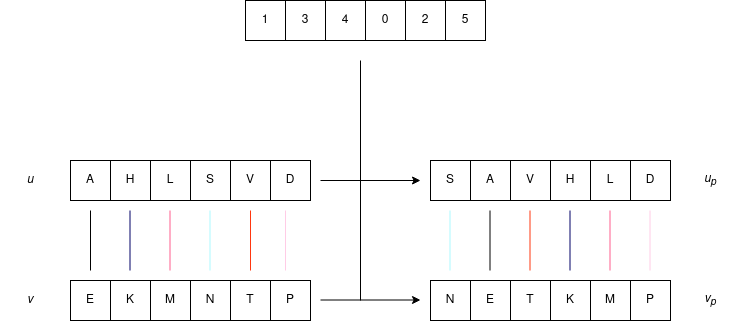
\includegraphics[scale=0.52]{graphics/shuffle.png}
\end{center}
\caption{Example of a permutation function and a graphical presentation of
the
sequence score invariance under permutation on both sequences.}
\label{fig:shuffle}
\end{figure}
\AVTcomment{The notation here is slightly different. I'll try to redo so
that
they are similar to text. Placeholder only.}
The sorting \(q\)-permutation \(\varphi_{u}\) is of special interest.
It sorts the characters in \(u\), i.e.\ it satisfies
\begin{align}
\Subchar{u}{\Perm{u}{i}}\leq\Subchar{u}{\Perm{u}{i+1}}\text{ for all }i,
0\leq
i\leq q-2
\end{align}
The resulting \Qgram{q} \(u_s=\varphi_{u}(u)\) is called sorted \Qgram{q}.
The inverse of \(\varphi_{u}\) is \(\varphi_{u}^{-1}\), defined by
\begin{align}
\Perminverse{u}{\Perm{u}{i}}=i\text{ for all }i, 0\leq i\leq q-1
\end{align}
As a consequence \(\Perminverse{u}{\Perm{u}{u}}=u\).
From the Lemma we can deduce, that it suffices to precompute the
the score tables \(\mathsf{ST}_{q'}\) for \(q'\in\{2,3\}\)
only for the sorted \(q'\)-grams. From these one can compute
the \(k\)-environment of a sorted \(q\)-gram whose members are finally
transformed by the inverse of the sorting permutation.
The advantage of this approach is the smaller number of sorted \Qgram{q}s
compared to unsorted, leading to a more efficient memory usage and a more
compacted computation of the score matrix. Table~\ref{tab:numdiff} outlines
the
difference in number of \Qgram{q}s to be enumerated and the size of the
resulted
score matrices.
\begin{table}
\begin{center}
\begin{tabular}{c|c|r|r|r}
type & \(q\) & Number & Score matrix & Matrix size ratio \\
& & of \Qgram{q}s & entries & \(\frac{|m_\text{sorted
\Qgram{q}}|}{|m_\text{unsorted \Qgram{q}}|}\)\\
\hline
\(q\)-grams & 2 & 400 & \numprint{160000} & 0.275625\\
Sorted \(q\)-grams & 2 & 210 & \numprint{44100} & \\
\hline
\(q\)-grams & 3 & \numprint{8000} & \numprint{64000000}& 0.3705625\\
Sorted \(q\)-grams& 3 & \numprint{1540} & \numprint{2371600}&
\end{tabular}
\caption{Number of \Qgram{q}s versus the number of sorted \(q\)-grams for
\(q\in\{2,3\}\) and an alphabet of size 20. The number of entries of the
the score matrix is calculated as the square of the number of (sorted)
\(q\)-grams.\label{tab:numdiff}}
\end{center}
\end{table}
\SKcomment{Here is an implementation issue which maybe should be discussed
in the corresponding section.
For the 210 sorted \(2\)-grams,
you need 8 bits to encode each, compared to 9 bits for the \(2\)-grams.
For the 1540 sorted \(3\)-grams,
you need 11 bits to encode each, compared to 13 bits for the \(3\)-grams.
This should at least be discussed at later, if encoding of \(2\)-grams
or \(3\)-grams becomes relevant in the implementation.}
\section{Working with sorted \Qgram{q}s}
\subsection{Enumeration}
In mathematics, a set is defined as a collection of items, where every
element occurs exactly once. This definition can be expanded to multisets,
where elements can occur more than once. Applying an order on these
multisets, we can formalize a notion of sorted \Qgram{q}s:
Given an alphabet \(\Alpha\) and a natural number \(q > 0\), a sorted
\Qgram{q} over \(\Alpha\) is a string \(u\in\Alpha^{q}\) such that
\(\Subchar{u}{i}\leq\Subchar{u}{i+1}\) for all \(i\), \(0\leq i\leq q-2\).
\SKcomment{As a multiset is a string, we should use the usual notation. So
I have rewritten the previous definition. Please apply the same scheme
below.}
The number of possible sorted \Qgram{q}s for a given \(\mathcal(A)\) and
\(q\) can be computed as the binomial \(\binom{q+r-1}{q}\) where
\(r=|\Alpha!\).
This can be proven by induction on \(q\)~\cite{pfn}.
The advantage of sorted \Qgram{q}s over normal \Qgram{q}s is that number of
sorted \Qgram{q}s is significantly smaller than the number of \Qgram{q}s
(see
Table~\ref{tab:numdiff}). Therefore, a separate index system is created to
map
every sorted \Qgram{q} sequentially to an integer, named sort code and
denoted
with \(sc\), i.e a function
\(sc: \Alpha^q \rightarrow [0,\binom{q+|\Alpha|-1}{q})\).
Firstly, an ordering must be defined on the set of all sorted \Qgram{q}s.
In
order for the ordering to comply with the usual \Qgram{q} encoding,
illustrated
in Equation~\ref{DefineHfunction}, we can define so
that if and only if a sorted \Qgram{q} \(u\) comes before \(v\),
the encoding of \(u\) is smaller than the encoding of \(v\):
\(i\) so that \(\Subchar{u}{i} < \Subchar{v}{i}\):
\begin{align}
\IT{q}{\Alpha}(u) < \IT{q}{\Alpha}(v)\Leftrightarrow H(u) < H(v)
\label{eq:ordering}
\end{align}
Using this definition, we can create a table to index every sorted
\Qgram{q},
i.e a table that assigns every sorted \Qgram{q} an index sequentially and
these
assigned indexes must follow Equation~\ref{eq:ordering}. A method to
compute
this table by enumerating every sorted \Qgram{q} is visualized in
Figure~\ref{fig:enumerate}.
\SKcomment{What do you mean by index table?}
\AVTcomment{Fixed. I hope this makes it clearer.}
Figure~\ref{fig:enumerate} showcases a model of the problem where \(q=5\)
and \(\Alpha=\{a_0,a_1,a_2\}\). If the prefix of length 2 of \(u\) is
fixed, say \(a_0a_1\), the last 3 characters are obtained as a sorted
\Qgram{q'} for \(q'=5-2=3\) and for the alphabet \(\Alpha'=\Alpha[a_1:]\).
The notation \(\Alpha[a_1:]\) denotes a subset of \(\Alpha\) containing
every
element \(a' \geq a_1\). Every character in \(\Alpha[a_1:]\) is placed in
the
third position of the \Qgram{q}, representing a further possibility of the
sequence. This idea can be generalized as follows:
Consider the construction of a sorted \Qgram{q} \(u\) of which the prefix
of
\(m\leq q\) characters has been determined and \(\Subchar{u}{m-1}=a_{i}\)
for
some \(i\), \(0\leq i\leq r-1\). Then
the task is to enumerate all sorted \Qgram{(q-m)}s over the alphabet
\(\Alpha_{i}=\{a_{i},a_{i+1},\ldots,a_{r-1}\}\). This process, presented as
a
recursive function, is outlined in
Algorithm~\ref{code:enumerateMultisetRec},
and the initial function call is
\(\mathsf{MultisetEnumerateRecursion}(q,\Alpha,'')\)
where \(''\) is the empty string.
\begin{figure}[t]
\begin{center}
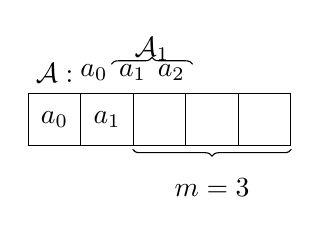
\begin{tikzpicture}
[arraynode/.style={inner sep=1pt,minimum height=19pt,minimum
width=19pt,rectangle,draw},
alphanode/.style={inner sep=1pt,minimum height=15pt,minimum
width=15pt,rectangle},
position label/.style={
below = 3pt,
text height = 1.5ex,
text depth = 1ex
},
overbrace/.style={decoration={brace},decorate},
underbrace/.style={decoration={brace,mirror},decorate}
]
\begin{scope}[start chain=1 going right,node distance=-0.5mm]
\node [alphanode,on chain=1] {\(\Alpha:\)};
\node [alphanode,on chain=1] {\FirstMultisetSymbol};
\node [alphanode,on chain=1] (A0) {\SecondMultisetSymbol};
\node [alphanode,on chain=1] (A1) {\ThirdMultisetSymbol};
\draw [overbrace,decoration={raise=-1ex}] (A0.north west) --
node [position label,yshift=2.5ex] {\(\Alpha_1\)} (A1.north east);
\end{scope}
\begin{scope}[shift={(0cm,-17pt)},start chain=2 going right,node
distance=-0.15mm]
\node [arraynode,on chain=2] {\FirstMultisetSymbol};
\node [arraynode,on chain=2] (Posb) {\SecondMultisetSymbol};
\node [arraynode,on chain=2] (N0) {};
\node [arraynode,on chain=2] {};
\node [arraynode,on chain=2] (N1) {};
\draw [underbrace,decoration={raise=1pt}] (N0.south west) --
node [position label,yshift=-1ex] {\(m=3\)} (N1.south east);
\end{scope}
\end{tikzpicture}
\end{center}
\caption{Example of enumerating sorted \Qgram{q}. Adapted from~\cite{pfn}}
\label{fig:enumerate}
\end{figure}
\begin{algorithm}[t]
\caption{Enumerating sorted \Qgram{q}s}
\label{code:enumerateMultisetRec}
\begin{tabular}{@{}l@{~}l}
\textbf{Input:}&current multiset length \(q'\)\\
&alphabet \(\Alpha\)\\
&current prefix \(u\)\\
&index table \(\IT{q}{\Alpha}\)
\end{tabular}
\begin{algorithmic}
\Function{\(\mathsf{MultisetEnumerateRecursion}(q',\Alpha',u)\)}{}
\If{\(q_i = 0\)}
\State \(\IT{q}{\Alpha}.\Append(u)\)
\Else
\For{\(a_j \in \Alpha'\)}
\State \(\mathsf{MultisetEnumerateRecursion}(q'-1,\Alpha[a_j:],ua_j)\)
\EndFor
\EndIf
\EndFunction
\end{algorithmic}
\end{algorithm}
\SKcomment{You do not refer to these algorithms, but your lemma refers to
table \(IT\) which likely stands for \(\IT{q}{\Alpha}\).}
\SKcomment{In Algorithm \ref{code:enumerateMultisetRec}
specify the recursive function using the keyword 'function' and
with its parameters, see for example, function approxmatch in
strees\_slides.pdf, in GIK. Do not use \(q_{i}\) and \(\Alpha_{i}\) as
Parameters, but \(q'\) and \(\Alpha\prime\). Instead of an alphabet
you should use an index to denote the index of the first of the remaining
characters. Then the alphabet is a global variable, represented as a list
of its ordered characters, and you can use the
slice notation to denote the list of remaining characters for iterate over
in the for-loop. Also the indextable can be considered a global variable.
As part
of algorithm \ref{code:enumerateMultisetRec} you specify that the initial
call is with \(q\) and the alphabet index \(0\).
Then Algorithm \ref{code:enumerateMultiset} becomes superfluous and
the initial can is to complicated anyway.}
\AVTcomment{I've fixed the naming. I'll also add 2 more direct step after
in
Figure~\ref{fig:enumerate} (placing \(a_1\) and \(a_2\) in the 3rd
position) to
make it clearer.}
\subsection{Linear encoding}
Using the index table, a scheme to encode any given \Qgram{q} over
alphabet \(\Alpha\) to its table index in \(O(q)\) can be devised.
\begin{Lemma}
\label{lm:weightproof}
There exists an unique integer weight for each character \(a\) in position
\(p\) so that given any sorted \Qgram{q} \(u\) over an alphabet
\(\Alpha\),
\begin{align}
c(u)=\sum_{p=0}^{q-1} w(p,u[p])\label{Equation:linearenc}
\end{align}
encodes exactly \(u\) to its index in table \(\IT{q}{\Alpha}\).
\begin{Proof}
\textbf{Base case:} In case of \(q=1\), \(|\Alpha|\) unigrams can be
clearly encoded with \(w(0,a) = a\) for all \(a \in \Alpha\).
\textbf{Inductive step:} Given the above scheme is valid up until
\(q-1\), \(q\in \Nats\), \(q\geq 2\), it needs to be shown that
\(w(q,a)\) is unique for
all \(a\in \Alpha\). Assuming the weight isn't unique, therefore there
exist two different weights \(w_a\neq w_a'\) so that \(c(au) = w_a + c(u)\)
and \(c(av) = w_a' + c(v)\) encode \Qgram{q}s \(au\) and \(av\)
respectively, \(u,v\in \Alpha^{q-1},a\in\Alpha\). The codes \(c(au)\) and
\(c(av)\) must but differ exactly the code of their suffixes \(c(u)-c(v)\),
since they share the same prefix. One can then formulate:
\begin{align}
sc(au) - sc(av) &= (w_a + sc(u)) - (w_a' + sc(v))\\
&= (w_a - w_a') + (sc(u) - sc(v))\\
&= sc(u) - sc(v)
\end{align}
which leads to \(w_a - w_a' = 0\), or \(w_a = w_a'\), which is a
contradiction. Therefore \(w(q,a)\) must be unique.
\end{Proof}
\end{Lemma}
\SKcomment{I think the lemma should be as below, as the main point is
the fact that \(c\) is bijective. The fact that \(w\) is unique does not
matter in my opionion. The proof should actually construct \(w\) and
show the bijective property.}
Lemma~\ref{lm:weightproof} then leads to the linear computation of the sort
code
\(sc\), outlined in Lemma~\ref{lm:codeproof}.
\begin{Lemma}
\label{lm:codeproof}
Let \(q>0\) and let \(M\) be the set of sorted \(q\)-grams over
alphabet \(\Alpha\). There is a function
\(w:\{0,\ldots,q-1\}\times\Alpha\to\Nats_{0}\), such that the function
\(sc:M\to\Nats_{0}\) defined by
\begin{align}
sc(u)=\sum_{p=0}^{q-1} w(p,\Subchar{u}{p})\label{Equation:linearenc}
\end{align}
satisfies
\begin{itemize}
\item \(sc(u)\in\{0,\ldots,|M|-1\}\) for all \(u\in M\) and
\item \(sc(u)\neq sc(u')\) for all \(u,u'\in M\), \(u\neq u'\).
\end{itemize}
\begin{Proof}
\AVTcomment{I must think about this proof a bit more.}
\end{Proof}
\end{Lemma}
The recursive method to compute a \(q\cdot r\)-table
LE is then derived from the proof above. The base case can be directly
given
and based on the index tables \(\mathsf{IT}_{q_i,\Alpha}\) for all
\(q_{i}\), \(2\leq q_i\leq q\).
\SKcomment{As you did not explain table \(\mathsf{IT}\), it
is impossible to follow your argumentation.}
the \Qgram{q_i}s are tracked for change in prefix and the weight of the
prefix can be calculated with Equation~\ref{Equation:linearenc}. The
pseudocode for the construction of LE is given in
Algorithm~\ref{code:linearEncodingTable}. The notation \([\bot] \times r\)
here
denotes the creation of a list of length \(r\) filled with empty values.
\begin{algorithm}[t]
\caption{Creating linear encoding table \(\LE{q}{\Alpha}\)}
\label{code:linearEncodingTable}
\begin{tabular}{@{}l@{~}l}
\textbf{Input:}&sequence length \(q\)\\
&alphabet \(\Alpha\) with size \(r\)\\
&index tables \(\text{IT}_{q',\Alpha}\text{ for all }q' \in [1,q]\)\\
\end{tabular}
\begin{algorithmic}
\State \(\LE{q}{\Alpha}\) \(\gets []\)
\State \(\LE{q}{\Alpha}.\Append(\{0,\ldots,r-1\}\))
\For{\(q'\in[2,q]\)}
\State \(\CurrentWeight \gets [\bot] \times r\)
\For{\(i,u\in\text{IT}_{q',\Alpha}\)}\Comment{Key-Value loop}
\If{\(\CurrentWeight [u[0]] = \bot\)}
\State \(\SuffixCode\gets \sum_{j=1}^{q'}\LE{q}{\Alpha}[j-1][u[j]]\)
\State \(\CurrentWeight [u[0]] \gets i - \SuffixCode\)
\EndIf
\EndFor
\State \(\LE{q}{\Alpha}.\mathsf{insert}(0,\CurrentWeight)\)\Comment{Place
more significant weight at beginning}
\EndFor
\end{algorithmic}
\end{algorithm}
\SKcomment{Apply all the remarks regarding naming and typesetting mentioned
before to Algorithm \ref{code:linearEncodingTable}.}
\SKcomment{In Algorithm \ref{code:linearEncodingTable} you only update
\(\CurrentWeight\) at index \(\Subchar{u}{i}\), which is likely not
correct.}
\AVTcomment{I've looked through the pseudocode again and compared to the
Python
script you provided. I think they look similar.}
\SKcomment{You introduce \(\CurrentWeight\) as a list of \(r\) elements
being undefined initially. So the insert-operation then prepends the value
of \(\CurrentWeight\) to \(\LE{q}{\Alpha}\). This should somehow be
commented.}
\SKcomment{I do not see why Algorithm \ref{code:linearEncodingTable} was
derived from the proof above. Need more explanation.}
\section{Simplified approach in determining the score-threshold}
\subsection{MMseqs and MMseqs2 approaches}
\SKcomment{You better use the section header 'determining the
score-threshold'.
The first subsection then describes how to derive a threshold given some
probability. The second subsection then describes how MMseqs determines
this probability. The subsection then describes your approach. In this
latter
subsection, you can to the first subsection after you have described your
derivation of \(p\).}
In MMseqs, in order to determine a proper score threshold \(k\),
a \(z\)-score statistics was applied. The program takes in an input \(s\)
from
user, which is labeled internally as the average \(k\)-environment size.
Unfortunately due to the unclear documentation, a thorough examination of
the
method was unsuccessful.
In MMseqs2, a heuristics was instead used,
where a base value was hardcoded and scaled back based on the user inputed
sensitivity value. For example, for searching using seed with weight 6, the
base
value was set to be 163.2 and the scaling factor for sensitivity was 8.917:
\begin{align}
k = \mathsf{base} - \mathsf{factor}\cdot s = 163.2 - 8.917 \cdot s
\end{align}
In order to test the accuracy of the threshold estimation, measurements
were firstly carried out on MMseqs2 with default seed.
\begin{figure}
\centering
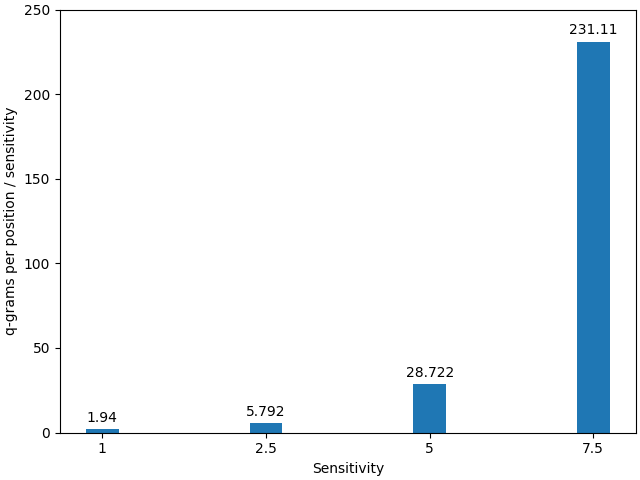
\includegraphics[scale=0.6]{graphics/mmseqs2_sensitivity.png}
\caption{Ratio of number of generated \Qgram{q}s using MMseqs2 approach
vs. expected}
\label{fig:mmseqssens}
\end{figure}
The test shows that MMseqs2 often overgenerated \Qgram{q}s, with the worst
case creating 231.11 times more than expected. Another observation on the
MMseqs2 approach is that as the base value is hardcoded, the threshold
estimation is not adaptive to the dataset. Therefore, the goal of this
section
is to provide a systematic approach that allows the user to control the
ammount
of \Qgram{q} generated more predictably and effectively.
\subsection{A simplistic approach}
In order to control the generation of \Qgram{q}s, a metric must firstly be
defined. The average environment size \(s\) was reused from MMseqs since
it's
a good metric that's intuitive to the user.
The average environment size \(s\) and the threshold \(k\) of the
environment can be related based on the tail
of a discrete distribution of scores for pairs of \(q\)-grams. So let
\(h_{q}(x)\) be the percentage of pairs
\((u,u')\in\Alpha^{q}\times\Alpha^{q}\) such that \(\sigma(u,u')=x\).
\SKcomment{Please check that this the correct definition of
\(h_{q}\). But you actually have plotted this only for a sample, but I
assumed
that the definition makes sense for the entire set of all \(q\)-grams.}
\AVTcomment{percentage would be more correct for distribution.}
\SKcomment{Just as a possible point for a discussion: The frequencies for
pairs of \(q\)-grams should be similar to the frequencies for sorted
\(q\)-grams.}
\SKcomment{Another possible point for a discussion: It should be possible
to calculate the exact distribution of the scores using a DP-method: Assume
integer scores. If one knows the distribution for all pairs of
\((q-1)\)-mers, then one can compute the distribution for all pairs of
\(q\)-grams. This would be an interesting GSA-exercise. I have just
added a Python-script \texttt{bin/pair\_score\_distrib.py}. Results look
okay,
but I have not verified them.}
\begin{figure}[t]
\begin{center}
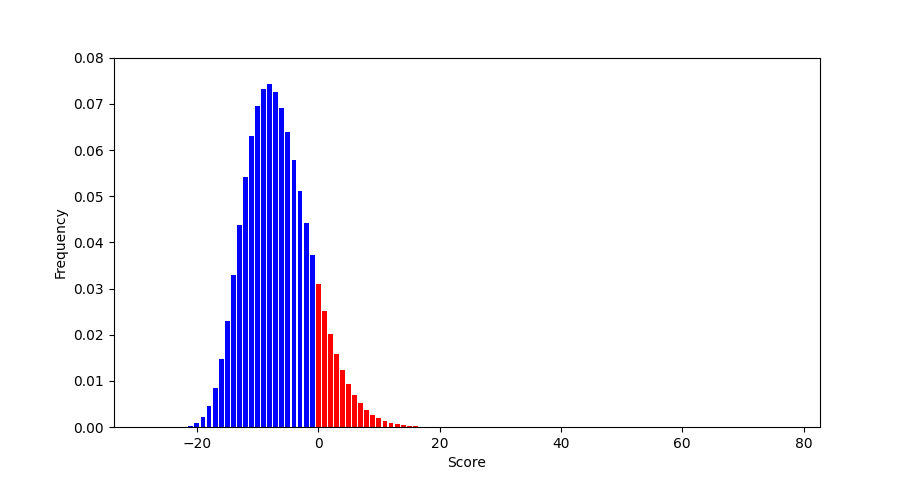
\includegraphics[scale=0.6]{graphics/distribution.png}
\end{center}
\caption{Estimated score distribution \(h_7\) between pairs of \Qgram{7}
using
BLOSUM62 score matrix and Equation~\ref{eq:convolution}. The character in
\Qgram{q}s \((h_1)\) are assumed to be uniformly distributed. The blue bars
show
the frequencies for events with
score \(<0\). The red bars show the frequencies for events with
score \(\geq 0\).}
\label{fig:distribution}
\end{figure}
Figure~\ref{fig:distribution} visualizes an exemplary score distribution
between uniformly distributed \Qgram{7}. The red portion in the right
tail describes the probability \(\mathcal{P}(\sigma \geq 0)\), which could
be generally quantified to:
\begin{align}
\mathcal{P}(\sigma \geq k) = \sum_{i = k}^\infty h_q(i)
\end{align}
The average environment size \(s\) could be normalized to
probability:
\SKcomment{So you assume an average size \(l\) of the \(k\)-environment and
to caluculate probability, which is suggested by the following equation,
as \(l\) appears on the right hand side of the equation.}
\begin{align}
p = \frac{s}{|\Alpha|^q}
\end{align}
Therefore threshold would be ideally in continuous
distribution equal to \(p\):
\SKcomment{Approximation of what? You have two equations with \(p\) on the
left hand side. The first is based on sampling the space of \(q\)-grams and
the second is based on an unkown probability function. Please be more
precise.
The current description is confusing.}
\begin{align}
p = \mathcal{P}(\sigma \geq k)
\end{align}
But since we have a discrete distribution of score values, we let \(p\) be
a
upper bound on probability:
\begin{align}
\mathcal{P}(\sigma \geq k) \leq p < \mathcal{P}(\sigma \geq
k-1)\label{eq:distribution}
\end{align}
The idea of the algorithm is to approximate a score distribution between
\Qgram{q} . Then the distribution can be iterated from the right tail to
calculate \(\mathcal{P}(\sigma \geq k)\), where \(k\) is the current score
threshold. The iteration can be stopped when Equation~\ref{eq:distribution}
is satisfied.
\SKcomment{According to my previous argumentation, you can determine
\(P(\sigma(u,v)\geq k\mid u,v\in\Alpha^{q})\) exactly from the
counts computed by \texttt{bin/pair\_score\_distrib.py}.}
Under the assumption that individual sequence characters follow a
context-free
model, i.e they occur independently from what comes before and after, the
score distribution between \Qgram{q}s \(h_q\) can be approximated
recursively
through convolution~\cite{dmsv}:
\begin{align}
h_{q}(x) = \sum_{y\in\mathcal{Z}} h_{q-1}(y)h_1(x-y)
\label{eq:convolution}
\end{align}
\SKcomment{So this is basically the idea which I used in
\texttt{bin/pair\_score\_distrib.py}. But why have you mentioned uniformly
distributed above, which refers to a sampling procedure. So you actually
have
not sampled the \(q\)-grams and computed the exact value? Actually, I
cannot
tell from you sloppy description.}
It is important to note that \(h_1\), the 1-gram score distribution,
depends on both character distribution collected from target sequence and
uniform character distribution. The reason is that the scores are between
\Qgram{q}s in query sequences and generated \Qgram{q}s. \Qgram{q}s in query
sequences can be assumed to follow the character distribution collected
from
target sequence, and the generated \Qgram{q}s follow the uniform character
distribution, since every characters in the generated \Qgram{q}s are
equally
likely to appear. The pseudocode for this computation is
summarized in Algorithm~\ref{code:ctxfree}.
\begin{algorithm}[t]
\caption{Approximation of an appropriate threshold \(k\) in context-free
approach}
\label{code:ctxfree}
\begin{tabular}{@{}l@{~}l}
\textbf{Input:}&single character distribution \(d\)\\
&score function \(\sigma\) with smallest and biggest score \(\Small\) and
\(\Biggg\)
respectively\\
&\Qgram{q} length \(q\)\\
&Alphabet size \(r = |\Alpha|\)\\
&Sensitivity, i.e average environment size \(s\)
\end{tabular}
\begin{algorithmic}
\State \(\PossibleValuesSingle \gets (\Biggg - \Small + 1)\)
\State \(\PossibleValuesTotal \gets \PossibleValuesSingle\cdot q\)
\State \(h_1 \gets [0] \times \PossibleValuesTotal\)
\For{\(c_1 \in \Alpha\)}
\For{\(c_2 \in \Alpha\)}
\State \(h_1[\sigma(c_1,c_2)-\Small]\text{ += }\frac{d[c_1]}{r}\)
\EndFor
\EndFor
\State \(h \gets h_1\)
\For{\(n \in [1,q)\)}\Comment{Convolute \(q-1\) times}
\State \(h_{\text{temp}} \gets [0] \times \PossibleValuesTotal\)
\For{\(i \in [0,\PossibleValuesSingle\cdot n)\)}
\For{\(j \in [0,\PossibleValuesSingle)\)}
\State \(h_{\text{temp}}[i+j]\text{ += }h[i]\cdot h_1[j]\)
\EndFor
\EndFor
\State \(h \gets h_{\text{temp}}\)
\EndFor
\State \(\Cutoff \gets \frac{s}{r^q}\)
\State \(i \gets \PossibleValuesTotal - 1\)
\State \(\Psum \gets 0\)
\While{\(i\neq 0\)}
\State \(\Psum\text{ += }h[i]\)
\If{\(\Psum > \Cutoff\)}
\State break
\EndIf
\State \(i \text{ -= }1\)
\EndWhile
\State return \(\Small \cdot q + i + 1\)
\end{algorithmic}
\end{algorithm}
\SKcomment{characters appeared in the environment? I do not understand.
The environment consists of \(q\)-grams. So you mean the characters in the
\(q\)-grams of the environment?}
\AVTcomment{yes}
\subsection{A more accurate estimation}
The above strategy treats single character as
independent and therefore loses its context in \Qgram{q}s, i.e what comes
before
and after. Another approach could then be hashing the target sequences to
collect \Qgram{q} distribution, which is convenient since the work is done
in
the processing of target dabase. This approach is but often complicated in
large \(q\), since a score matrix between pairs of \Qgram{q}s must be
computed,
which incurs an additional penalty of \(O(|\Alpha|^{2q})\), which is often
infeasible when \(q>4\).
A middle ground is to divide the \Qgram{q}s
into two or three shorter segments, possibly similar to the branch and
bound
algorithm in Section~\ref{section:qgramgen}, and collect their positional
distribution separately, i.e the number of distributions corresponds
directly to
number of segments, regardless of their length.
\begin{algorithm}[t]
\caption{More accurate threshold estimation (Part 1): Extract hash values}
\label{code:ctxsens1}
\begin{tabular}{@{}l@{~}l}
\textbf{Input:}&vector of hash value \(\HashValVec\)\\
&score function \(\sigma\) with smallest and biggest score \(\Small\) and
\(\Biggg\)
respectively\\
&\Qgram{q} length \(q\)\\
&Alphabet size \(r = |\Alpha|\)\\
&Sensitivity, i.e average environment size \(s\)
\end{tabular}
\begin{algorithmic}
\State \(\ModFactors \gets []\)
\State \(\DivFactors \gets []\)
\For{\(i\in[0,|\Qsplit(q)|)\)}\Comment{Create factors to extract hash value
of small segments}
\State \(\ModFactors.\Append(r^{\Qsplit(q)[i]})\)
\State \(\DivFactor \gets 1\)
\For{\(j\in[i+1,|\Qsplit(q)|)\)}
\State \(\DivFactor\text{ \(\cdot\)= }\Qsplit(q)[j]\)
\EndFor
\State \(\DivFactors.\Append(\DivFactor)\)
\EndFor
\State \(d \gets []\)
\For{\(i\in[0,|\Qsplit(q)|)\)}\Comment{Extract hash values of segments}
\State \(d.\Append([0] \times \ModFactors[i])\)
\EndFor
\For{\(\HashValue\in\HashValVec\)}
\For{\(i\in[0,|\Qsplit(q)|)\)}
\State \(\HashValue_i \gets (\frac{\HashValue}{\DivFactors[i]}) \%
\ModFactors[i]\)\Comment{Integer division}
\State \(d[i][\HashValue_i]\text{ += }1\)
\EndFor
\EndFor
\end{algorithmic}
\end{algorithm}
The key idea of Algorithm~\ref{code:ctxsens1} is that based on
Equation~\ref{DefineHfunction}, the hash values of the \Qgram{q} \(u\) can
be
treated as an \(q\) digit long \(r\)-ary number \((r=|\Alpha|)\), where the
\(i\)-th character in the \Qgram{q} corresponds to the \(i\)-th digit in
the
number. Therefore, to extract the hash value of the substring
\(\Subchar{u}{i\ldots j}\), \(0 \leq i \leq j < q\), one can first apply a
right shift, which corresponds to an integer division. Thereafter, an
modulo
operation with the operand \(r^{j-i+1}\) was used, which is extracts the
last
\(j-i+1\) digits (corresponding to the substring).
\AVTcomment{Maybe a figure here is needed to represent the extraction.}
After the positional hash values are extracted, they are collected to
create
their individual histogram. The histograms then get normalized to
distribution
and the distributions are convoluted together to approximate the \Qgram{q}
distribution. The extraction of
threshold \(k\) then follows the same approach in the simplistic approach.
The
pseudocode for this computation is
summarized in Algorithm~\ref{code:ctxsens}.
\begin{algorithm}[t]
\caption{More accurate threshold estimation (Part 2): Creating score
distribution and extract threshold}
\label{code:ctxsens}
\begin{algorithmic}
\State \(\PossibleValuesSingle \gets (\Biggg - \Small + 1)\)
\State \(\PossibleValuesTotal \gets \PossibleValuesSingle\cdot q\)
\State \(h_b \gets []\)
\For{\(i\in[0,|\Qsplit(q)|)\)}\Comment{Collect score distribution}
\State \(h_b.\Append([0] \times \PossibleValuesTotal)\)
\For{\(\HashValue_1\in[0,\ModFactors[i])\)}
\For{\(\HashValue_2\in[0,\ModFactors[i])\)}
\State \(h_b[i][m_{\Qsplit(q)[i]}[\HashValue_1][\HashValue_2]]\text{ +=
}\frac{d[i]}{\ModFactors[i]}\)
\EndFor
\EndFor
\EndFor
\For{\(i\in[0,|\Qsplit(q)|)\)}\Comment{Normalize distribution}
\For{\(j\in[0,\PossibleValuesTotal)\)}
\State \(h_b[i][j]\text{ /= }\HashValVec.\mathsf{length}\)
\EndFor
\EndFor
\State \(h \gets h_b[0]\)
\State \(\ell\gets \Qsplit(q)[0]\)
\For{\(n \in [1,|\Qsplit(q)|)\)}\Comment{Convolute \(|\Qsplit(q)|-1\)
times}
\State \(h_{\text{temp}} \gets [0] \times \PossibleValuesTotal\)
\For{\(i \in [0,\PossibleValuesSingle\cdot \ell)\)}
\For{\(j \in [0,\PossibleValuesSingle\cdot \Qsplit(q)[n])\)}
\State \(h_{\text{temp}}[i+j]\text{ += }h[i]\cdot h_b[n][j]\)
\EndFor
\EndFor
\State \(\ell\text{ += }\Qsplit(q)[n]\)
\State \(h \gets h_{\text{temp}}\)
\EndFor
\State \(\Cutoff \gets \frac{s}{r^q}\)
\State \(i \gets \PossibleValuesTotal - 1\)
\State \(\Psum \gets 0\)
\While{\(i\neq 0\)}
\State \(\Psum\text{ += }h[i]\)
\If{\(\Psum > \Cutoff\)}
\State break
\EndIf
\State \(i \text{ -= }1\)
\EndWhile
\State return \(\Small \cdot q + i + 1\)
\end{algorithmic}
\end{algorithm}
\SKcomment{Please be more precise: same approach as what? I assume you want
to state, that derivation of \(k\) is as in the context dependent approach
of section \ref{}.}
\AVTcomment{I have renamed the approach to not mention context. I'll still need
a name to refer to each approach in Result section. Can you recommend me how to 
call them?}

\Chapter{Implementation and Design}
\section{Design overview}

The program consists of seven main classes:

\SKcomment{Which program? Invent a name, say SuperMMseqs, and then start as
follows: Most of the methods described above where implemented in a program
SuperMMseqs. The implementation in C++ followed an object oriented approach,
makes heavy use of Metaprogramming and is based on the following
seven main classes:}

\begin{enumerate}
\item A seed reader to convert a spaced seed specification into a binary
representation and to compute the span and weight of the spaced seed.
To further process seeds, two variants are created:

\SKcomment{Variants of what?}

\SKcomment{seeds are not processed. They have been converted before. But the
sequences are processed.}

\begin{enumerate}
\item Target reader divides seeds into blocks of shorter \Qgram{q}s as
input for recursive hashing function.

\item Query reader divides seeds into blocks of short segments, sorts query
sequences and uses sorted \Qgram{q} encoder to linearly encode the
resulted sorted \Qgram{q}s.
\end{enumerate}

\SKcomment{The reader do not divide anything. They only extract \(q\)
characters from the input sequences at positions specified by the space seed.}

\item A recursive hash engine to collect every \Qgram{q} hashes from
target sequences and package them.

\SKcomment{The verb packages has not been used before. If you write 'every'
you cannot use 'hashes'. Please be more precise and consistent in your wording.}
\item A sorted \Qgram{q} index table to index every sorted \Qgram{q} for a
given scoring function and \(q\).

\SKcomment{As \(q\) is also use for the target reader and the query reader,
it does not make sense to only introduce it here. Also the scoring function
should be introduced before. How is this represented in your code?}

\item Sorted \Qgram{q} encoder creates a table to help linearly encode
sorted \Qgram{q}s.
\item A class to approximate an appropriate threshold given target sequence
data.
\item A score matrix to cache all scores between sorted \Qgram{q}s and
unsorted \Qgram{q}s.
\item An environment constructor gets sorted \Qgram{q} codes from the
query seed reader, uses them to call individual scores from the score
matrices and generates a Cartesian product from the environments.
\end{enumerate}

\SKcomment{Unclear what 'call individual scores from the score matrices'.
I assume the at environment constructor can process any code of a
sorted q-gram and is not dependent on the query seed reader.}

\SKcomment{Why do you need to cache scores between sorted \Qgram{q}s and
unsorted \Qgram{q}s. Or do you mean for pairs of sorted \(q\)-qgrams and
for pairs of unsorted \(q\)-qgrams?}

\SKcomment{As remarked earlier, the Query reader must also apply a
recursive hashing function. This comes before the sorting I guess.}

\SKcomment{Blocks of short segments is redundant. Blocks would suffice.
Do not use the notion of segments here. When you later consider
sorted matching seeds of two seqnum/position pairs, then the notion of
segment becomes relevant. That is, a segment consists of all matching seeds
for the same pair of target/query sequence.}

In Figure~\ref{fig:classes}, the relationship and dataflow between the
classes are outlined. Since the implementation of the recursive hashing of
target sequences is straightforward and does not diverge much from the
pseudocode, the section below focuses mainly on the processing of query
sequences.

\SKcomment{Usually when you show diagrams in which the nodes represent
classes, the edges represent dependencies of the code. That is when,
there is an edge from class A to class B, then B uses must know the class
name B and
the public instance variables and methods. This does not necessariy coincide
with the data flow. Accordung to your version you mix relation ships
(class B knows class A) and dataflow. But all edges could also represent
the data flow. Does it coincide with the class dependencies?}

\SKcomment{I assume that the ellipses represent input data
and the edge going out from ellipses represent the data flow. If this is
correct you need to add a second directed edge from target sequence to
threshold estimator.}
\SKcomment{Please specify what a rhombus means and a rectangle means. Likely
intediat data and result data. But there is no class which joins the target
hash data and the query environments to obtain match data.}
\SKcomment{Why use 'hash' in 'target hash data' but not in 'query data'? After
all, the elements delivered by the environment constructor re hashed as well.}

\begin{figure}[t]
\begin{center}
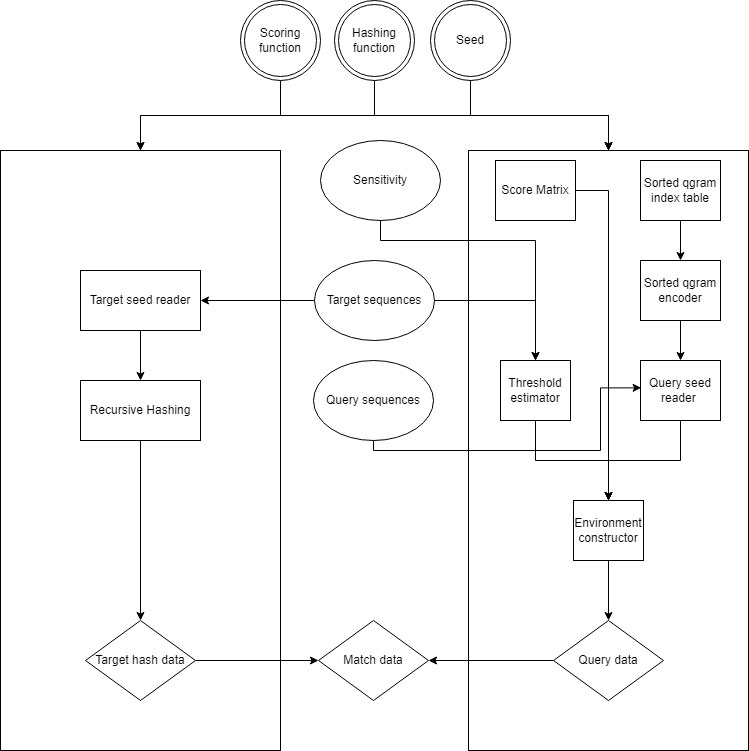
\includegraphics[scale=0.5]{graphics/Class_Diagram.png}
\end{center}
\caption{Relationship between the main classes and inputs}
\label{fig:classes}
\end{figure}


\section{Input}
At compile time, the program takes in a scoring function, which in the
context of protein sequences could be a BLOSUM or PAM matrix, a spaced seed
and a recursive hashing function. The scoring function should detail the

\SKcomment{You cannot descibe an assumption using the word 'should'. Also
put the information in appropriate order. So just write:
The scoring function consists of a matrix
of scores for each pair of characters from a given alphabet. This alphabet
is referenced in the scoring function. The alphabet provides a rank function
to encode each of its characters as a unique integer.}

relevant alphabet, the transformer function, which encodes every character
in the alphabet to its corresponding rank, and a matrix of scores between
every pairs of characters. Internally, the spaced seed is initially
represented as a numeric constant,

\SKcomment{constant of which type?}

\SKcomment{In the table in which you show the spaced seeds used, you do not
show the leading and trailing zeros. But if you represent a spaced seed as a
constant, you have to have some convention. The most promiment is:
All spaced seed begin with a 1 and end with a 1. This would allow to reprent
the spaced seed anywhere in a 64-bit unsigned integer. But you likely represent
the spaced seed right aligned. This means that the span is defined by
the position of the most signicant 1 bit.}

which during computation will be
transcoded into a bitset. The span of the seed can then be computed
according to the position of the first {1 in} the bitset and also the seed
weight \(q\) is the number of 1 bits.

At run time the program takes in two set of sequences in FASTA format.
Any data error, for example empty file or corrupt data format will
automatically lead to termination of the program and an error message will
be logged~\cite{gttl}. Additionally, the sensitivity of the program can be
adjusted as a command line argument.

\section{Compile time computation}
Figure~\ref{fig:classes} shows that some classes/tables can be evaluated at
compile time.

\SKcomment{How can I derive this from figure~\ref{fig:classes}?}

Each seed gets transcoded and its weight and span can be

\SKcomment{What is transcoded? Previously you mentioned binary encoded.
Likely you mean the same.}

precomputed and therefore, the two seed readers and their schematics can be

\SKcomment{What is the schematiasc of a seed reader?}

predetermined. The two index tables for sorted/unsorted 2-grams/3-grams
take in only scoring function as parameter and therefore, can be complete be
computed at compile time. Since the linear encoding table LE (see
Algorithm~\ref{code:linearEncodingTable}) is based solely on the sorted
2-grams/3-grams index table, it also can be evaluated at compilation.

\SKcomment{How do you sort at compile time? Possibly std::sort can sort
a std::array at compile time, but as you do not specify how the tables are
stored, one can only guess. But such details are neceesary for the
description of the implementation.}

\SKcomment{The index table do not take in
the scoring function. They are based on the scoring function. Please be more
precise.}

\section{Run time computation}
At run time, at first the target and query database gets encoded using the
transformer function. Using the target seed reader, the target sequences
are then hashed in \(O(nb)\) time and the hashes are packaged as
byte units and saved in a contiguous container (i.e.\ array or vector).

\SKcomment{It must be a vector, as for an array you would need its size
at compile time.}
In the processing of query sequences, firstly the \Qgram{2} and \Qgram{3}
score matrices \(\Scoretablename\) can be evaluated using the index tables

\SKcomment{Please do not write 'can be evaluated'. Use 'are evaluated'}

\SKcomment{Why are the \Qgram{2} and \Qgram{3} matrices \underline{evaluated}?
They have been computed at compile time, i.e.\ for each \(2\)-gram and
\(3\)-gram \(u\) one can enumerate \(2/3\)-gram/score-pairs \((v,\sigma(u,v))\)
in sorted order.}

from sorted and unsorted \Qgram{q}s according to
Equation~\ref{equation:sequenceScore}.

\SKcomment{Why from sorted to unsorted \(q\)-grams? The evaluation was
defined for \(q\)-grams. So it applies to sorted \(q\)-grams as well.}

The result then can then be stored
as a pair of score and unsorted \Qgram{q} code and sorted after score
value for further use.

\SKcomment{So you mean the \(k\)-environment for a single \(q\)-gram
can be stored and sorted? But that does not make sense since on below
you explain how to determine the score-threshold. I am lost.}

Thereafter, an appropriate threshold is evaluated
using the target sequences and an user-provided sensitivity. Using the
score matrices and the threshold, the program enters the step of \Qgram{q}
generation using the Cartesian product.

\subsection{Local composition bias correction}
MMseqs2 employs a mechanism to evaluate the positional
context of an amino acid when processing the query sequences. The
idea of this mechanism is to adjust the score threshold \(k\)
for regions whose local amino acid composition varies
considerably from the background distribution. Without adjusting, these low
regions can lead to biases in the prefiltering result. This correction of
the threshold can be summarized as follow:

\begin{align}
\Delta \sigma_i(u[i]) =
\underbrace{\sum_{a\in \Alpha}f(a)\sigma(a,\Subchar{u}{i})}_{\text{expected score}}-
\underbrace{\frac{1}{2d}\sum_{j=i-d,j\neq i}^{i+d}\sigma (u[i],u[j])}_{\text{average local score}}
\end{align}

\SKcomment{The bias depends on the position, so that the amino acid is
implicitely given. This should be reflected in the notation and one
should define it as \(\Delta(i)\) or \(\Delta(\sigma,u,i)\).}

where \(u\) is the query sequence, \(i\) is the current position in the
sequence, \(d\) is a positive integer (explained below)
and \(f(a)\) is the background frequency of residue \(a\).

\SKcomment{\(d\) is not defined and I assume that \(i\geq d\) and
\(i+d\leq |u|-1\) must hold. You define it later, but it should be mentioned
here (which I did.)}

The minuend is a representation of

\SKcomment{I do not like the notion of minuend, as to me it is not clear what
it means. From the context one can deduce that it is
the first sum. So better write. The expression
\(\sum_{a\in \Alpha}f(a)\sigma(a,\Subchar{u}{i})\) is
the expected score resulting from the
background distribution of the amino acids. For each \(b\in\Alpha\) one can
precompute \(\sum_{a\in \Alpha}f(a)\sigma(a,b)\) given \(f\).}

The subtrahend involves the current region in the query sequence and
introduces a parameter \(d\) for the radius of the region, defined in
MMseqs2 as a constant 20.

\SKcomment{Do not use the notion subtrahend. Use 'the term which is
subtracted' is an average local score at position \(i\) involving \(d\)
amino acids on the left and on the right.}

The corrected score between a query \Qgram{q} \(u\) and its generated
\Qgram{q} \(v\) can then be computed as the sum of the pairwise amino acid
score and the score correction.

\begin{align}
\sigma_c(u,v) = \sigma (u,v) + \sum_{i=0}^{q-1} \sigma_i(u[i])
\end{align}

\SKcomment{Replace \(\sigma_i(u[i])\) using the notation as suggested above.}

In the implementation, this correction is instead subtracted from the
threshold at the beginning of the computation

\SKcomment{beginning of the computation of what? Like of \(\sigma(u,v\).
One should be more specific about the context in which this computation
occurs. You only state that it is applied when processing the query sequence.
But one should be more precise, as the evaluation becomes relevant
when the \(k\)-environment is constructed for the \(q\)-gram at position
\(i\). So actually becomes a \(k_{c}\)-environment is constructed.}

\begin{align}
\sigma_c(u,v) = \sigma (u,v) + \sum_{i=0}^{q-1} \sigma_i(u[i]) \geq k
\Leftrightarrow \sigma (u,v) \geq k - \sum_{i=0}^{q-1} \sigma_i(u[i]) =
k_{c}
\end{align}

\subsection{Turning Wheel Mechanism}
An issue in enumerating the Cartesian product is the possible difference in
the number of loops (e.g.\ 2 loops for seed weight 4-6, 3 loops for seed weight
7). To resolve this problem and allow easy expansion to greater seed
weight, a flexible loop structure is designed, where an array containing
the loop indexes is created. The earliest entry of the array holds the
outermost loop index and the later an entry is, the more inner the loop
index the entry holds. By iterating through only the innermost loop and
only adjusting the outer loop indexes as needed, the scheme can account for
any number of loops.
The formulation of the loop structure, is outlined in the
Algorithm~\ref{code:turningWheel}.

\SKcomment{The three function in Algorithm~\ref{code:turningWheel} are
not defined and explained. It is important to note the \(\mathsf{getScore}\)
computase the score from wheel and with respect to the \(q\)-gram which is
the input to the algorithm. For this it requires access to the loop data vector.
You have also not explained what the elements of
the loop data vector are. These are the elements of the sets to build
the cartesian product for. You also can merge the two lines
\(\Code \gets \mathsf{getCode}(\Wheel);\)
\(\mathsf{createQgram}(\Code)\) into one and introduce a function which
computes the \(q\)-gram from the wheel. It should be clarified that
creating a \(q\)-gram involves applying the reverse of the sorting permutation
and results into an element of the \(k\) environment.}

\SKcomment{I actually do not see the point of merging the turning wheels code
with the specific application of generating elements from the \
\(k\)-mer environment. I would keep the abtract view which only requires
to provide the sizes of each of the sets to construct the
cartesian product from and an abstract function which is applied to the
wheel.}

\SKcomment{I do not understand why you could end a loop or not even
turn the wheel, if you obtain a score \(<k\) This is only possible,
if the elements in the data vector are sorted by the score, which has not been
mentioned. This feature could also be integrated into the abstract function
mentioned above.}

\begin{algorithm}[t]
\caption{Turning Wheel Mechanism}
\label{code:turningWheel}
\begin{tabular}{@{}l@{~}l}
\textbf{Input:}&number of loops \(n\)\\
&loop data vector \(v_0\), \(v_1\), ..., \(v_{n-1}\)\\
&threshold \(k\)\\
&function \(\mathsf{createQgram}\)\\
&function \(\mathsf{getScore}\)\\
&function \(\mathsf{getCode}\)
\end{tabular}
\begin{algorithmic}
\State \(\Loopid \gets n-1\)
\State \(\Wheel \gets [0]\times n\)
\State \(\Score \gets \mathsf{getScore}(\Wheel)\)
\If{\(\Score < k\)} \Comment{Current data vectors not viable. Early
Termination.}
\State return
\Else \Comment{First loop iteration}
\State \(\Code \gets \mathsf{getCode}(\Wheel)\)
\State \(\mathsf{createQgram}(\Code)\)
\EndIf
\While{True}
\State \(\Wheel[\Loopid]\gets \Wheel[\Loopid]+1\)
\If{\(\Wheel[\Loopid] \geq \text{len}(v_{\Loopid})\)}\Comment{End of loop}
\State \(\Wheel[\Loopid] \gets 0\)
\If{\(\Loopid = 0\)}\Comment{No longer viable in outermost loop}
\State break
\EndIf
\State \(\Loopid\gets \Loopid-1\)
\Else
\State \(\Score \gets \mathsf{getScore}(\Wheel)\)
\If{\(\Score \geq k\)}\Comment{Viable \Qgram{q} found}
\State \(\Code \gets \mathsf{getCode}(\Wheel)\)
\State \(\mathsf{createQgram}(\Code)\)
\Else \Comment{No viable \Qgram{q} found, end current loop}
\State \(\Wheel[\Loopid]\gets \text{len}(v_{\Loopid})\)
\EndIf
\If{\(\Loopid \neq n-1\)}\Comment{Reset to innermost loop}
\State \(\Loopid \gets n-1\)
\EndIf
\EndIf
\EndWhile
\end{algorithmic}
\end{algorithm}
\begin{comment}
\subsection{SIMD}
SIMD (Single-Instruction Multiple-Data) is a group of instructions allowing
vectorized, parallel data processing. Instead of processing data
sequentially, they are capable of defining wide registers, commonly 128-bit
or 256-bit, packaging data in those registers and process data in parallel.
The key to the shuffle using SIMD is the instruction
\(\mathsf{\_\_mm\_shuffle\_epi8}\), which is available on platforms
supporting
SSSE3 instruction sets or the equivalent \(\mathsf{vqtbl1q\_u8}\) on ARM
platform. Both instructions take in two 128-bit (equivalent to 16-byte)
vectors.
In order to comply with the instructions, both the \Qgram{q} and the
inverse
permutation get padded internally to 16-byte. First vector holds the data,
in
this case the \Qgram{q}, and the second the information on how the data get
shuffled, in this case the inverse permutation.
\begin{figure}[t]
\begin{center}
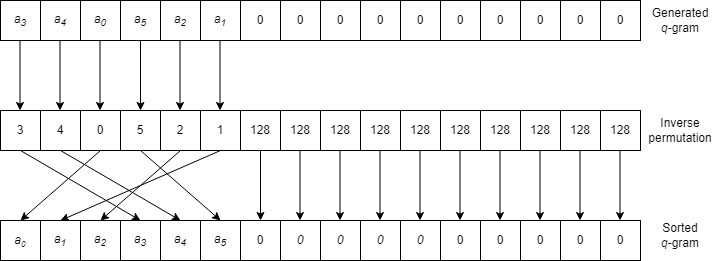
\includegraphics[scale=0.6]{graphics/SIMD.png}
\end{center}
\caption{Schematics of SIMD instruction \_\_mm\_shuffle\_epi8}
\label{fig:simd}
\end{figure}
A schematic is visualized in Figure~\ref{fig:simd}. The right padded
section of the inverse permutation is filled with integer 128 to signal the
instruction to not shuffle and to simply pad the resulted vector with 0.
\end{comment}
\section{Merging target and query data}
After being collected, the hashed data from all target and query sequences
is packaged as byte units, prioritizing hash values.

\SKcomment{Unclear what prioritizing means here. You basically store the
hash-value in the most significant bits and then are sorted taking only the
number of bits used for the hash value. So they are basically sorted
by hash-values.}

They then get sorted
individually using radix sort,

\SKcomment{What does sorted individually mean here?}

resulting in two data vectors sorted by hash
values which would then be merged value by value, skipping through
unmatching blocks.
\begin{algorithm}[t]
\caption{Merging query and target data}
\label{code:merging_data}
\begin{tabular}{@{}l@{~}l}
\textbf{Input:}&query data \(\Query\)\\
&target data \(\Target\)\\
&function \(\mathsf{CreateMatch}\)
\end{tabular}
\begin{algorithmic}
\State \(\TargetIdx \gets 0\)
\State \(\QueryIdx \gets 0\)
\While{\(\TargetIdx \neq \Target.\End\) \(\text{ and }\) \(\QueryIdx \neq
\Query.\End\)}
\State \(\HashValue_t \gets \Target[\TargetIdx].\HashValue\)
\State \(\HashValue_q \gets \Query[\QueryIdx].\HashValue\)
\If{\(\HashValue_t < \HashValue_q\)} \Comment{Skipping on target vector}
\While{\(\Target[\TargetIdx].\HashValue = \HashValue_t\)}
\State \(\TargetIdx\gets\TargetIdx+1\)
\EndWhile
\Else
\If{\(\HashValue_t > \HashValue_q\)} \Comment{Skipping on query vector}
\While{\(\Query[\QueryIdx].\HashValue = \HashValue_q\)}
\State \(\QueryIdx\gets\QueryIdx+1\)
\EndWhile
\Else \Comment{Match found}
\State \(\TBlockEnd = \TargetIdx\)
\While{\(\Target[\TBlockEnd] = \HashValue_t\)}
\State \(\TBlockEnd\gets\TBlockEnd+1\)
\EndWhile
\State \(\QBlockEnd = \QueryIdx\)
\While{\(\Query[\QBlockEnd] = \HashValue_q\)}
\State \(\QBlockEnd\gets\QBlockEnd+1\)
\EndWhile
\State
\(\mathsf{CreateMatch}([\TargetIdx,\TBlockEnd),[\QueryIdx,\QBlockEnd))\)
\State \(\TargetIdx\gets\TBlockEnd\)
\State \(\QueryIdx\gets\QBlockEnd\)
\EndIf
\EndIf
\EndWhile
\end{algorithmic}
\end{algorithm}

\SKcomment{Algorithm \ref{code:merging_data} looks good, but it should be
referenced from the main text.}

The merging process results in a vector of matches, represented again as
byte units, containing respectively the sequence number of the match on the
target, on the query, the diagonal number (difference between the target
and query sequence position), and the query sequence position. These
quartets are again sorted with radix sort to prepare for ungapped alignment
stage.

\SKcomment{You better mention that the matches are used for prefiltering:
Only if a segment contains a diagonal with at least two matches, it is
processed further with the ungapped alignment algorithm.}

\Chapter{Benchmark and Performance}
Separate modular benchmarks were carried out for the processing of target
sequences, threshold estimation and similar \Qgram{q} generation. All
measurements were performed using C++ on an Intel CPU i5-\numprint{10300}H
2.5~GHz with 8~GB DDR4 running Ubuntu on a SSD. The program was compiled
with
g++ 11.3.0.
The test dataset composed of a target database from MMseqs2 and a query
database created as a difference set from MMseqs2 queryset against the
target database. Some statistics on these datasets are summarized below in
Table~\ref{tab:datasets}. The scoring function used in testing is the
BLOSUM62
score matrix.
\section{Processing target sequences}
Testing from Figure~\ref{fig:target_hashing} showed that the direct
extraction of \Qgram{q}s generally has a better run time, as expected from
Table~\ref{tab:seeds}. Even the hashing using seed \numprint{111011}, which
was
predicted to have performance speedup, failed to show improvement. The
reason
could be repeated lookup of character to remove/add causing cache-miss,
slowing
the computation.
\begin{figure}[t]
\begin{center}
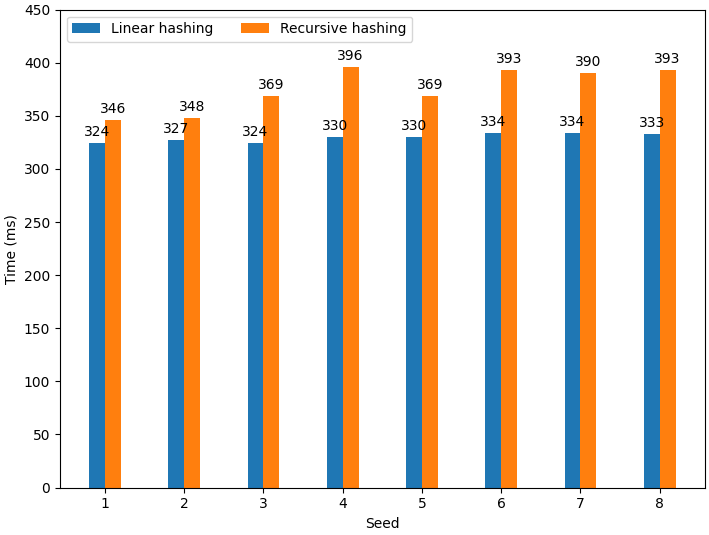
\includegraphics[scale=0.45]{graphics/target_hashing.png}
\end{center}
\caption{Performance of two hashing functions}
\label{fig:target_hashing}
\end{figure}
\section{Determining threshold}
In order to test the accuracy of the threshold estimation, measurements
were firstly carried out on MMseqs2 with default seed.
\begin{figure}
\centering
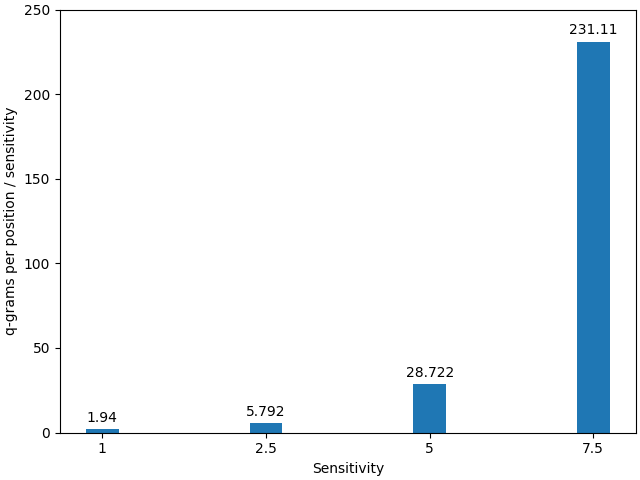
\includegraphics[scale=0.6]{graphics/mmseqs2_sensitivity.png}
\caption{Ratio of number of generated \Qgram{q}s using MMseqs2 approach
vs. expected}
\label{fig:mmseqssens}
\end{figure}
The test shows that MMseqs2 often overgenerated \Qgram{q}s, with the worst
case creating 231.11 times more than expected.
Both of the approaches, context-free and context-sensitive, were tested
with the
dividing scheme in context-sensitive approach reused from the \Qgram{q}
generation algorithm. For each test, the total number of \Qgram{q}s
generated is
averaged and then compared to the expected list length per position and
MMseqs2
result.
\begin{figure}
\centering
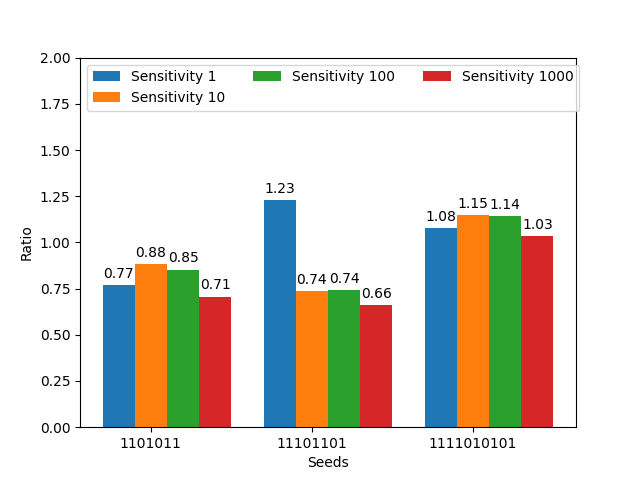
\includegraphics[scale=0.6]{graphics/threshold_contextfree.png}
\caption{Ratio of number of generated \Qgram{q}s using context-free
approach vs. expected}
\label{fig:numctxfree}
\end{figure}
\begin{figure}
\centering
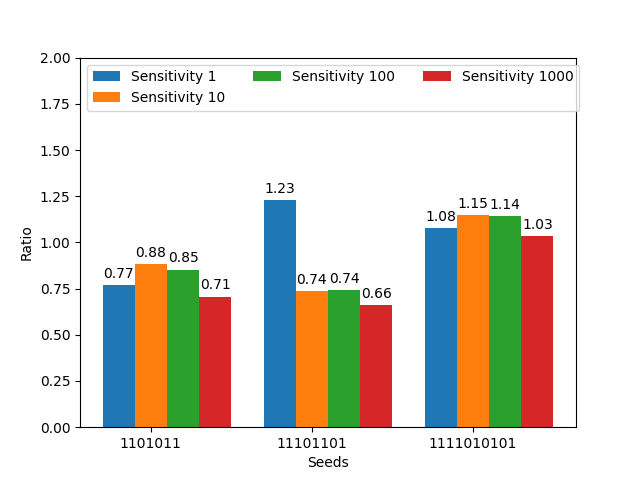
\includegraphics[scale=0.6]{graphics/threshold_contextsens.png}
\caption{Ratio of number of generated \Qgram{q}s using context-free
approach vs. expected}
\label{fig:numctxsens}
\end{figure}
The benchmarks of context-free (Figure~\ref{fig:numctxfree}) and
context-sensitive approach (Figure~\ref{fig:numctxsens}) both show better
control compared to MMseqs2 and the resulted list lengths are relatively
close to the expected value. The thresholds created by this approach show
to be a good upper bounds for the \(k\)-environment in lower \(q\), where
only sensitivity of 1 in the seed weight 6 crosses the expected ammount. In
higher seed weight, both approaches serve well as an approximation, where
only a maximum of 15~\% more \Qgram{q}s were generated compared to
expected value.
It's also noticeable that both approaches result in the same
threshold, which could be due to the relatively short sub-\Qgram{q} length.
Since the dividing schema in the branch-and-bound algorithm is reused,
histograms
of \Qgram{2} and \Qgram{3} were created and due to their small length, they
are
not sufficient to diverge from the character distribution used in
context-free
approach. In order to discern the usage of each approach,the run time
of each method is investigated further in Figure~\ref{fig:sens_runtime}:
\begin{figure}
\centering
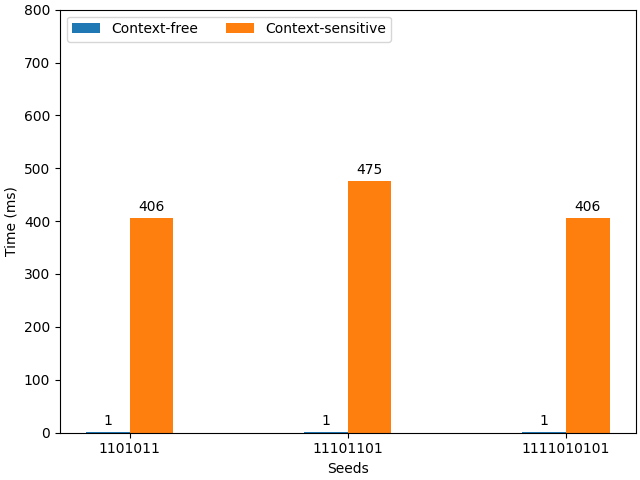
\includegraphics[scale=0.6]{graphics/speed_threshold.png}
\caption{Run time comparison of context-free vs. context-sensitive
approach}
\label{fig:sens_runtime}
\end{figure}
The context-free approach shows to take very little time, almost
instantaneous.
Coupled with the very good estimation of the threshold it proves to be an
universal on-the-fly solution. The context-sensitive approach takes a lot
more
time, average around 0.5~s to create a threshold (compensated for creation
of
unsorted-unsorted \Qgram{q} score matrices, see
Section~\ref{section:scorematrix}),since it incurs a \(O(|\Alpha|^{2q})\)
time to build histogram. Therefore this approach should be used only on
high sensitivity, where long computation time is expected, or cached in the
preprocessing of target sequences.
It is important to note that since the approximation of the threshold \(k\)
doesn't take local score correction into account, all of the above
measurements are without local score correction. In
Figure~\ref{fig:compbias} are some benchmarks with correction of varying
degree, showcasing how the average list length is impacted. The result
shows that the average \Qgram{q} list can vary strongly and unpredictably
under usage of local composition bias score correction, where if the scale
of the correction is from 0.75~-~1, the resulted number can be as few as 5
times or as many as 48 times more than expected. The proper scaling of the
factor remains to be investigated further.
\begin{figure}
\centering
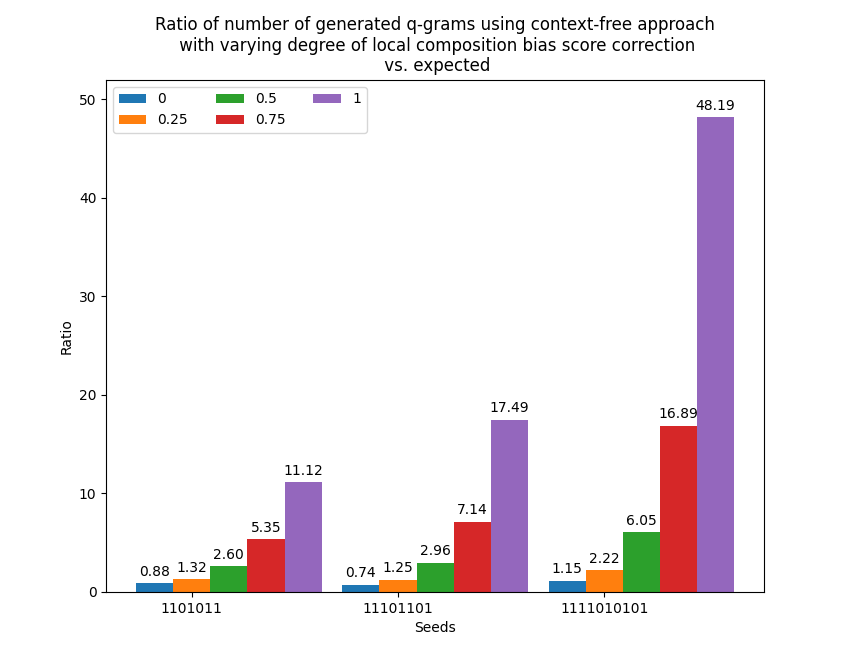
\includegraphics[scale=0.6]{graphics/comp_bias.png}
\caption{Influence of local composition bias score correction on average
\Qgram{q} list length. The original estimation on \Qgram{q} list length
was 10.}
\label{fig:compbias}
\end{figure}
\section{Generating \Qgram{q}s}
In order to test the efficiency of the \Qgram{q} list generation, the
original workflow in MMseqs2 was replicated and tested against the new
algorithm. This workflow, along with both variants of the new algorithm,
with and without SIMD implementation, was measured in
Figure~\ref{fig:genw5}, \ref{fig:genw6} and \ref{fig:genw7} for different
seed weights.
\begin{figure}
\centering
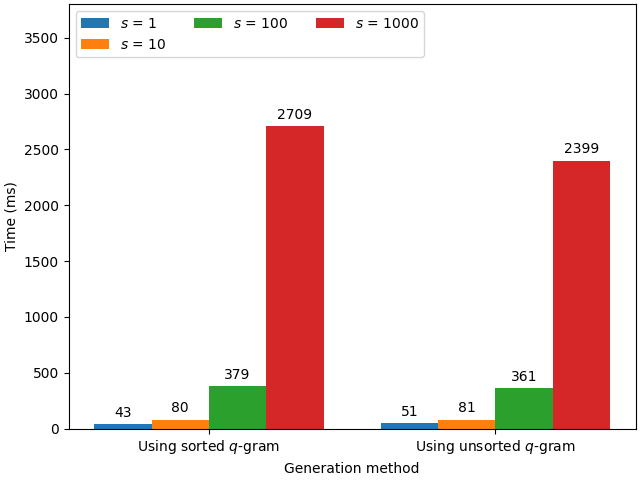
\includegraphics[scale=0.6]{graphics/gen_w5.png}
\caption{Time measured in miliseconds to generate \Qgram{q}s with
different sensitivities using seed \numprint{1101011}}
\label{fig:genw5}
\end{figure}
\begin{figure}
\centering
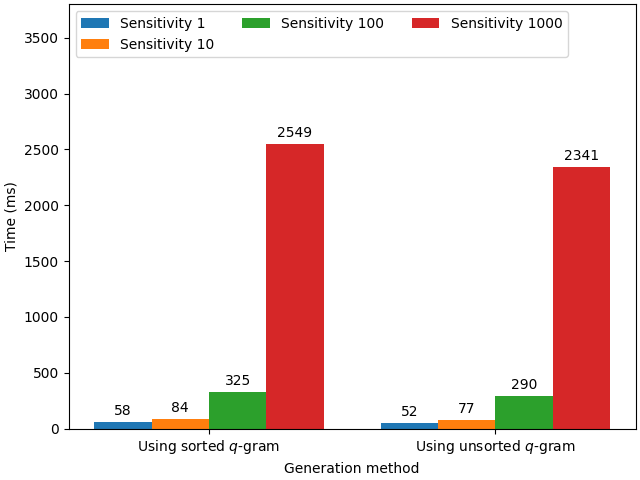
\includegraphics[scale=0.6]{graphics/gen_w6.png}
\caption{Time measured in miliseconds to generate \Qgram{q}s with
different sensitivities using seed \numprint{11101101}}
\label{fig:genw6}
\end{figure}
\begin{figure}
\centering
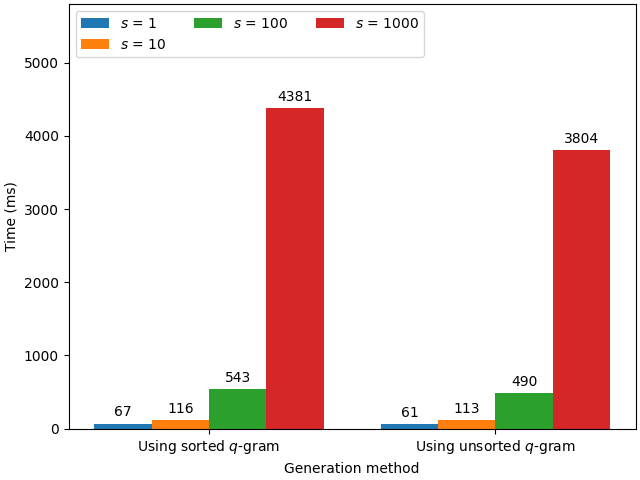
\includegraphics[scale=0.6]{graphics/gen_w7.png}
\caption{Time measured in miliseconds to generate \Qgram{q}s with
different sensitivities using seed \numprint{1111010101}}
\label{fig:genw7}
\end{figure}
The tests showed that the new algorithm has generally a 10~\% to 15~\%
performance loss compared to the MMseqs2 method. This is the overhead
caused by the sorting and reshuffled of \Qgram{q}. The tradeoff is the low
initial memory consumption, where only 340~MB of memory is consumed for the
score matrices instead of 1.80~GB (see Table~\ref{tab:memdiff}).
\begin{table}
\begin{center}
\begin{tabular}{c|c|}
\Qgram{q} type & Memory Allocated in Bytes\\
\hline
Using sorted \Qgram{q}s & 340704000\\
Using sorted \Qgram{q}s & 1811500000\\
\end{tabular}
\caption{Comparison of initial memory footprints in creation of score
matrices
between two approaches. Data collected using Intel
V-Tune.\label{tab:memdiff}}
\end{center}
\end{table}
On average, the
program spends 18.2~ns to generate a \Qgram{5}, 18.3~ns to generate a
\Qgram{6} and 20.1~ns to generate a \Qgram{7}. This shows that the
\Qgram{q}
generation scales generally well with \(q\), where an additional loop in
creation of \Qgram{7} causing an increase of 10~\% in run time. It could
then
be reasoned that the generation of \Qgram{8} and \Qgram{9} may follow the
same
trend, which coupled with the new approach in estimating threshold could
lead to
an expansion of seed weight (see Section~\ref{section:expand}).
\section{General Performance}
In this section, the overall run time of the whole program is profiled to
find hotspots and to figure the scalability of the system. The program will
be run with the most optimized settings, meaning context-free threshold
approximation and \Qgram{q} generation using sorted method. In Figure, the
recorded time in each step of the program is visualized.
\begin{figure}
\centering
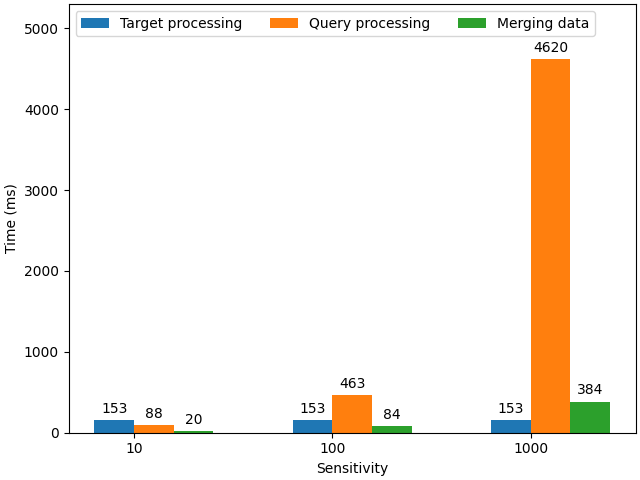
\includegraphics[scale=0.6]{graphics/program_w6.png}
\caption{Run time of different phases in the program, measured in
miliseconds,
using seed \numprint{11101101}, sensitivity 10, 100 and \numprint{1000}}
\label{fig:program_w6}
\end{figure}
\begin{figure}
\centering
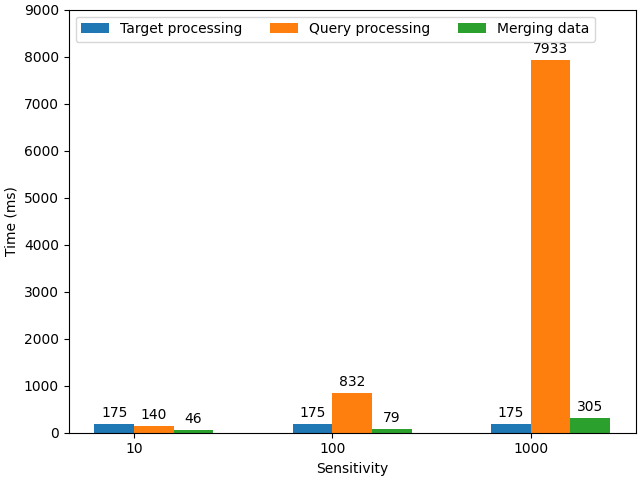
\includegraphics[scale=0.6]{graphics/program_w7.png}
\caption{Run time of different phases in the program, measured in
miliseconds,
using seed \numprint{1111010101}, sensitivity 10, 100 and \numprint{1000}}
\label{fig:program_w7}
\end{figure}
The test showed that the run time of processing target data is generally
negligible. The processing of match data could be more significant,
reaching
0.4~s in testing but still scales much better than \Qgram{q} generation
phase.
This means that the hotspot of the program lies in the \Qgram{q} generation
phase, specifically in the Cartesian product formation and in lesser
manner,
the radix sort of \Qgram{q} data. In the most heavy measurement, the
\Qgram{q}
generation phase still takes 1.5~-~2 times as long as the sorting after,
see
Figure~\ref{fig:hotspot_w6} and \ref{fig:hotspot_w7}.
\begin{figure}
\centering
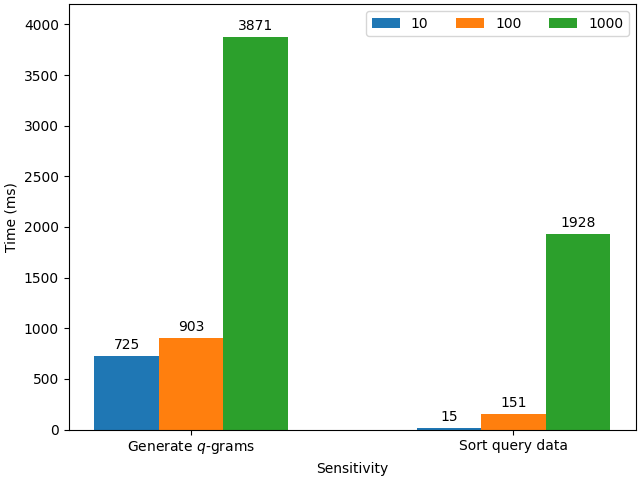
\includegraphics[scale=0.6]{graphics/hotspot_w6.png}
\caption{Run time of \Qgram{q} generation and radix sort, measured in
miliseconds,
using seed \numprint{11101101}, sensitivity 10, 100 and \numprint{1000}}
\label{fig:hotspot_w6}
\end{figure}
\begin{figure}
\centering
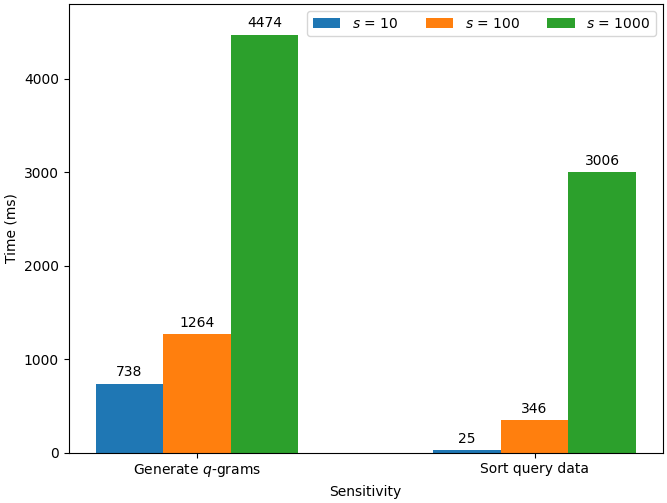
\includegraphics[scale=0.6]{graphics/hotspot_w7.png}
\caption{Run time of \Qgram{q} generation and radix sort, measured in
miliseconds,
using seed \numprint{1111010101}, sensitivity 10, 100 and \numprint{1000}}
\label{fig:hotspot_w7}
\end{figure}
\Chapter{Discussion \& Future improvements}
\section{Performance}
The performance of the implementation using both sorted and unsorted
\Qgram{q}s
is compared to MMseqs2 in Figure~\ref{fig:mmseqs2comp}.
\begin{figure}
\centering
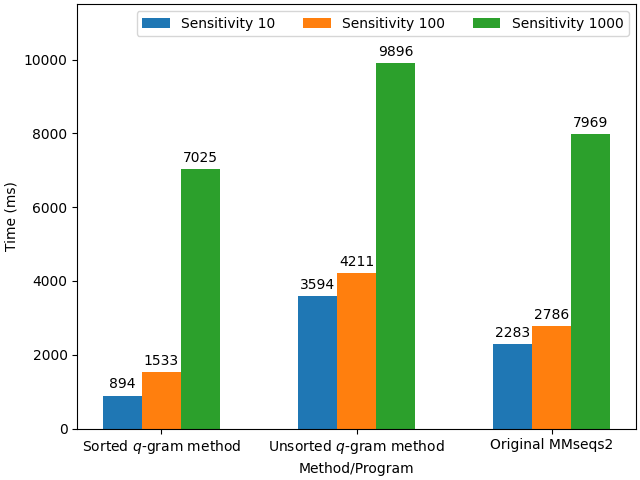
\includegraphics[scale=0.6]{graphics/mmseqs2comp.png}
\caption{Run time of the program using both sorted and unsorted \Qgram{q}s,
measured in ms, is compared to MMseqs2, in generation of 10, 100 and 1000
\Qgram{q} per sequence position}
\label{fig:mmseqs2comp}
\end{figure}
Compared to the MMseqs2 program, the implementation using unsorted
\Qgram{q}s
shows generally worse performance, with ... more time taken. On the other
hand,
the approach using sorted \Qgram{q}s presents better run time, especially
in
lower sensitivity. This shows that using optimization methods implemented
in
MMseqs2 could improve the run time even further.
Two further possible optimization methods are usage of SIMD intructions and
multithreadsing. Both of these methods were tried in the implementation
using
SIMD instruction \(\mathsf{\_\_mm\_shuffle\_epi8}\) and OpenMP library, but
unfortunately both showed little to no improvement on run time. Reasons for
these behaviors remains to be investigated.
\section{Features}
The new workflow was created with expandability in mind, therefore a lot of
the calculation allows for greater seed size and even greater sub-\Qgram{q}
size. A few of MMseqs2 features were also recreated, namely the ability to
scale local composition bias correction and sensitivity manually. The
design of the program also prioritizes flexibility, in that every
calculation option, ranging from MMseqs2 mode vs new sorted \Qgram{q}
method mode and both context-free and context-sensitive approach can be
changed on-the-fly without recompilation.
The program was intended to be a testing environment only, therefore custom
workflows in MMseqs2 were not recreated, namely the stepwise sensitive
search.
\section{Possibility of expanding seed\label{section:expand}}
Earlier it was shown that the run time of \Qgram{q} generation scales
almost constantly to seed, therefore some testing was created to test for
seeds of weight 8 and 9:
\AVTcomment{Waiting for BytesUnit fix}
\section{Compile-time calculation of
score matrices\label{section:scorematrix}}
Even though the class diagram in Figure~\ref{fig:classes} shows that it's
possible to compute the score matrix in compile time, since it only depends
on the two index tables of sorted/unsorted \Qgram{q}s, the implementation
decides to create the table in run time instead. The reason largely is due
to the high memory stack size requirements and lack of compile time sorting
algorithm. A manual compile time sorting implementation (i.e.\ quicksort)
would again demand more compile time instances. A separate benchmark in
Figure~\ref{fig:scorematrix} showed that this could incur a 0.6~s loss in
creating the sorted-unsorted \Qgram{3} score matrix or 3.3~s in creating
the unsorted-unsorted \Qgram{3} score matrix at the start of the
computation.
\begin{figure}
\centering
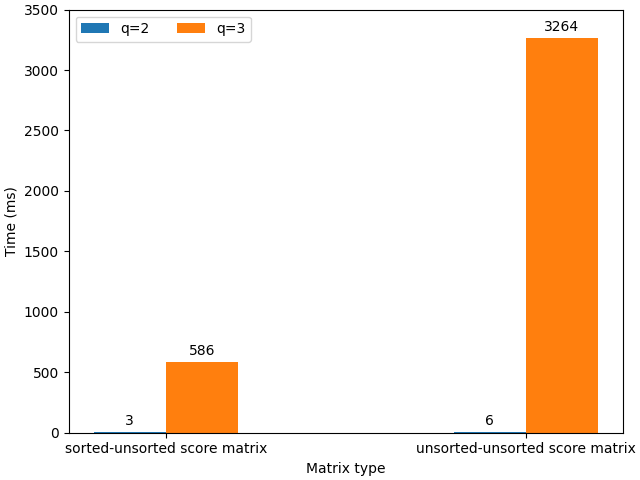
\includegraphics[scale=0.7]{graphics/scorematrix.png}
\caption{Time measured in miliseconds to generate \(q\times q\) score
matrix}
\label{fig:scorematrix}
\end{figure}
\Chapter{Conclusion}
In this paper, the prefiltering module of the MMseqs2 software suite was
examined and alternative optimization methods were tried and tested. A
possible improvement in processing target sequences through recursive
hashing, although has a better time complexity in theory, was shown to not
be a major improvement, other than in edge cases of low block numbers. A
new method of estimating threshold for better estimation of number of
generated \Qgram{q}s was implemented and showed to be a better estimation
approach, both in low and high sensitivity. Finally, an optimized
branch-and-bound algorithm was introduced and presented a lower memory
consumption in tradeoff for marginal increase in run time, allowing future
expansion into larger seed size.
%%%%<
%bibliography
\newpage
\small
% change the name of the bib-file to get your own bibliography
\bibliographystyle{unsrt}
\bibliography{template}
\normalsize

%%%%>
% appendix
\appendix
\noappendicestocpagenum
\addappheadtotoc
\Chapter{Some additional method descriptions}
\begin{table}
\begin{center}
\begin{tabular}{c|c|c|c}
Dataset & Number of sequences & Maximum Sequence Length & Minimum Sequence
Length\\
\hline
QUERY\_DIFF & 426 & \numprint{4291} & 8\\
TARGET & \numprint{20000} & \numprint{8081} & 7\\
\end{tabular}
\caption{Datasets used in testing the modules\label{tab:datasets}}
\end{center}
\end{table}

\Chapter{Some Additional Data}
%%%%<
\Assertion
\end{document}
